%------------------------------------------------------------------------------------------%
%------------------------------------------------------------------------------------------%
%------------------------------------------------------------------------------------------%
%                                      FILE BEGINS
%------------------------------------------------------------------------------------------%
%------------------------------------------------------------------------------------------%
%------------------------------------------------------------------------------------------%

%------------------------------------------------------------------------------------------%
%------------------------------------------------------------------------------------------%
%                                    DOCUMENT CLASS
%------------------------------------------------------------------------------------------%
%------------------------------------------------------------------------------------------%
\documentclass[a4paper]{jpconf}

%------------------------------------------------------------------------------------------%
%------------------------------------------------------------------------------------------%
%                                       PACKAGES
%------------------------------------------------------------------------------------------%
%------------------------------------------------------------------------------------------%
\usepackage{amsmath}
\usepackage{booktabs}
\usepackage{cite}
\usepackage{float}
\usepackage{graphicx}
\usepackage[caption=false]{subfig}
\usepackage[makeroom]{cancel}

%------------------------------------------------------------------------------------------%
%------------------------------------------------------------------------------------------%
%                                    DOCUMENT BEGINS
%------------------------------------------------------------------------------------------%
%------------------------------------------------------------------------------------------%
\begin{document}

%------------------------------------------------------------------------------------------%
%                                        HEADER
%------------------------------------------------------------------------------------------%

\title{Computing energy release rates using the Virtual Crack Closure Technique with the Finite Element Method: analytical discussion}

\author{Luca Di Stasio$^{1,2,a}$ , Janis Varna$^{2,b}$ and Zoubir Ayadi$^{1,c}$ }

\address{$^{1}$SI2M, IJL, EEIGM, Universit\'e de Lorraine, 6 Rue Bastien Lepage, F-54010 Nancy, France\\$^{2}$Division of Polymer Engineering, Lule\aa\ University of Technology, SE-97187 Lule\aa , Sweden }

{\vspace*{5pt}\address{E-mail: $^{a}$luca.di-stasio@univ-lorraine.fr, $^{b}$janis.varna@ltu.se, $^{c}$zoubir.ayadi@univ-lorraine.fr}}
%\address{$^{a}$luca.di-stasio@univ-lorraine.fr}, \address{$^{b}$janis.varna@ltu.se}, \address{$^{c}$zoubir.ayadi@univ-lorraine.fr}

%------------------------------------------------------------------------------------------%
%                                       ABSTRACT
%------------------------------------------------------------------------------------------%

\begin{abstract}
The effect of debond size and crack tip orientation of mode splitting in the Virtual Crack Closure Technique is analyzed by means of analytical derivations.
\begin{enumerate}
\item The total energy release rate is shown to have no direct dependence on the debond angular size, but only an indirect one through the FEM solution of the crack displacement field in the crack tip neighborhood. It thus can be computed using unrotated forces and displacements, i.e. aligned with the global and not with the local refere
\item Mode I and mode II energy release rate are expressed as a function of the crack displacement and it is shown as in \cite{Valvo:2012} that crack tip forces depend linearly on both components of the crack displacements. However, what in \cite{Valvo:2012} is an assumption used to reverse-engineer the relationship, here the dependency is fully derived in terms of the underlying FEM discretization. It is furthermore shown that crack tip forces do not only depend on crack displacements, but also on the resultant of forces of the 4 elements connected to the crack tip, which represent the influence of the rest of the domain.
\item A new vectorial formulation of the VCCT is proposed, which can be applied to elements of different order and in the presence of quarter-tip singularity (based on the work in \cite{raju:}). It provides a general framework for the analysis of curved cracks analyzed with FEM. It furthermore expresses directly the dependence on FEM discretization and solution. By implementing the equations provided alongside the classic FEM, it can provide a native formulation which does not to the extraction of internal or reaction forces in the post-processing phase.
\item It is shown that mode I and mode II for a curved crack behaves as $A\log\left(\delta\right)+B$, where $\delta$ is the angular discretization at the crack tip. The result is confirmed by the numerical results.
\end{enumerate}
\end{abstract}

%------------------------------------------------------------------------------------------%
%                                   List of acronyms
%------------------------------------------------------------------------------------------%

\section*{List of acronyms}

\begin{tabular}{ll}
VCCT &  Virtual Crack Closure Technique\\
BEM &  Boundary Element Method\\
FEM &  Finite Element Method\\
\end{tabular}
%\end{table}

%------------------------------------------------------------------------------------------%
%                                   List of symbols
%------------------------------------------------------------------------------------------%

\section*{List of symbols}

%\begin{table}[!h]
\begin{tabular}{lcl}
$G_{I}$ & $\left[\frac{J}{m^{2}}\right]$  & Mode I energy release rate\\
$G_{II}$ & $\left[\frac{J}{m^{2}}\right]$  & Mode II energy release rate\\
$G_{TOT}$ & $\left[\frac{J}{m^{2}}\right]$  & Total energy release rate\\
$G_{I,r\theta}$ & $\left[\frac{J}{m^{2}}\right]$  & Mode I energy release rate in $r-\theta$ reference frame\\
$G_{II,r\theta}$ & $\left[\frac{J}{m^{2}}\right]$  & Mode II energy release rate in $r-\theta$ reference frame\\
$G_{TOT,r\theta}$ & $\left[\frac{J}{m^{2}}\right]$  & Total energy release rate in $r-\theta$ reference frame\\
$\widetilde{G}_{I,xy}$ & $\left[\frac{J}{m^{2}}\right]$  & Mode I energy release rate of equivalent crack in $x-y$ reference frame\\
$\widetilde{G}_{II,xy}$ & $\left[\frac{J}{m^{2}}\right]$  & Mode II energy release rate of equivalent crack in $x-y$ reference frame\\
$\widetilde{G}_{TOT,xy}$ & $\left[\frac{J}{m^{2}}\right]$  & Total energy release rate of equivalent crack in $x-y$ reference frame\\
$R_{f}$ & $\left[\mu m\right]$  &Fiber radius\\
$a$ & $\left[\mu m\right]$  &Debond size\\
$\Delta a$ & $\left[\mu m\right]$  &Debond increment\\
$\Delta\theta$ & $\left[rad\right]$  & Half debond angular size\\
$\delta$ & $\left[rad\right]$  & Angular size of element at the interface close to the crack tip\\
$u_{x,[A-Z]}$ & $\left[\mu m\right]$  & Displacement along $x$ of a point labeled with a letter in [A-Z]\\
$u_{y,[A-Z]}$ & $\left[\mu m\right]$  & Displacement along $y$ of a point labeled with a letter in [A-Z]\\
$u_{x}$ & $\left[\mu m\right]$  & Displacement along $x$-direction\\
$u_{y}$ & $\left[\mu m\right]$  & Displacement along $y$-direction\\
$u_{r}$ & $\left[\mu m\right]$  & Displacement along $r$-direction\\
$u_{\theta}$ & $\left[\mu m\right]$  & Displacement along $\theta$-direction\\
$F_{x,[A-Z]}$ & $\left[\mu m\right]$  & Force along $x$ at a point labeled with a letter in [A-Z]\\
$F_{y,[A-Z]}$ & $\left[\mu m\right]$  & Force along $y$ at a point labeled with a letter in [A-Z]\\
$F_{x}$ & $\left[\mu m\right]$  & Force along $x$-direction\\
$F_{y}$ & $\left[\mu m\right]$  & Force along $y$-direction\\
$F_{r}$ & $\left[\mu m\right]$  & Force along $r$-direction\\
$F_{\theta}$ & $\left[\mu m\right]$  & Force along $\theta$-direction\\
$\underline{\underline{R}}$ & $\left[-\right]$  & Rotation matrix\\
\end{tabular}
%\end{table}

\clearpage
%------------------------------------------------------------------------------------------%
%                        FEM formulation with quadrilateral elements
%------------------------------------------------------------------------------------------%
\section{ FEM formulation with quadrilateral elements}

\begin{equation}
\Pi\left(u_{i}\right)=\int_{V}\sigma_{ij}\varepsilon_{ij}dV+\int_{V}\rho\ddot{u}_{i}u_{i}dV-\int_{V}F^{T}_{i}u_{i}dV-\int_{S}f^{T}_{i}u_{i}dS
\end{equation}

\begin{equation}
\Pi\left(u_{i}\right)=\int_{V}\sigma_{ij}\varepsilon_{ij}dV-\int_{V}F^{T}_{i}u_{i}dV-\int_{S}f^{T}_{i}u_{i}dS
\end{equation}

\begin{equation}
\varepsilon_{ij}=\frac{1}{2}\left(u_{i,j}+u_{j,i}\right)
\end{equation}

\begin{equation}
\underline{\varepsilon}\left(x,y\right)=\underline{\underline{\widetilde{B}}}\cdot\underline{u}\left(x,y\right)
\end{equation}

\begin{equation}
\underline{\widetilde{B}}=\begin{bmatrix}
\frac{\partial }{\partial x}&0\\[7.5pt]
0&\frac{\partial }{\partial y}\\[7.5pt]
\frac{\partial }{\partial y}&\frac{\partial }{\partial x}\\
\end{bmatrix}
\end{equation}

%\begin{equation}
%\underline{\varepsilon}\left(x,y\right)=\underline{\underline{\widetilde{B}}}\cdot\underline{u}\left(x,y\right)=\underline{\underline{\widetilde{B}}}\cdot\underline{\underline{N}}\cdot\underline{u}_{N}=\underline{\underline{B}}\cdot\underline{u}_{N}
%\end{equation}

\begin{equation}
\underline{\sigma}=\underline{\underline{D}}\cdot\underline{\varepsilon}
\end{equation}

\begin{equation}
\underline{\sigma}=\begin{bmatrix}
\sigma_{xx}\\\sigma_{yy}\\\tau_{xy}
\end{bmatrix}\qquad\underline{\varepsilon}=\begin{bmatrix}
\varepsilon_{xx}\\\varepsilon_{yy}\\\gamma_{xy}
\end{bmatrix}
\end{equation}

\begin{equation}
\underline{\underline{D}}=\begin{bmatrix}
E_{1}&E_{2}&0\\E_{2}&E_{1}&0\\0&0&G
\end{bmatrix}\qquad\text{with }G=\frac{E}{2\left(1+\nu\right)}\text{ for an isotropic material}
\end{equation}

\begin{equation}
\begin{split}
E_{1}=\frac{E}{1-\nu^{2}}\quad E_{2}=\nu E_{1}\quad&\text{for plane stress}\\
E_{1}=\frac{E\left(1-\nu\right)}{\left(1+\nu\right)\left(1-2\nu\right)}\quad E_{2}=\frac{\nu E_{1}}{1-\nu}\quad&\text{for plane strain}
\end{split}
\end{equation}

\begin{equation}
\begin{split}
\Pi\left(\underline{u}\right)=&\frac{1}{2}\int_{V}\underline{\underline{\varepsilon}}^{T}\underline{\underline{D}}\cdot\underline{\underline{\varepsilon}}dV-\int_{V}\underline{F}^{T}\underline{u}dV-\int_{S}\underline{f}^{T}\underline{u}dS=\\
&=\frac{1}{2}\int_{V}\underline{u}^{T}\underline{\underline{\widetilde{B}}}^{T}\underline{\underline{D}}\cdot\underline{\underline{\widetilde{B}}}\cdot\underline{u}dV-\int_{V}\underline{F}^{T}\underline{u}dV-\int_{S}\underline{f}^{T}\underline{u}dS
\end{split}
\end{equation}

\begin{equation}
\delta\Pi\left(\delta\underline{u}\right)=0
\end{equation}

\begin{equation}
\begin{split}
\delta\Pi\left(\delta\underline{u}\right)=&\Pi\left(\underline{u}+\delta\underline{u}\right)-\Pi\left(\underline{u}\right)=\\=&\frac{1}{2}\int_{V}\left(\underline{u}+\underline{\delta u}\right)^{T}\underline{\underline{\widetilde{B}}}^{T}\underline{\underline{D}}\cdot\underline{\underline{\widetilde{B}}}\cdot\left(\underline{u}+\underline{\delta u}\right)dV-\int_{V}\underline{F}^{T}\left(\underline{u}+\underline{\delta u}\right)dV-\int_{S}\underline{f}^{T}\left(\underline{u}+\underline{\delta u}\right)dS+\\
-&\frac{1}{2}\int_{V}\underline{u}^{T}\underline{\underline{\widetilde{B}}}^{T}\underline{\underline{D}}\cdot\underline{\underline{\widetilde{B}}}\cdot\underline{u}dV+\int_{V}\underline{F}^{T}\underline{u}dV+\int_{S}\underline{f}^{T}\underline{u}dS=\\
=&\cancel{\frac{1}{2}\int_{V}\underline{u}^{T}\underline{\underline{\widetilde{B}}}^{T}\underline{\underline{D}}\cdot\underline{\underline{\widetilde{B}}}\cdot\underline{u}dV}+\cancelto{\approx 0}{\frac{1}{2}\int_{V}\underline{\delta u}^{T}\underline{\underline{\widetilde{B}}}^{T}\underline{\underline{D}}\cdot\underline{\underline{\widetilde{B}}}\cdot\underline{\delta u}dV}+\\
+&\frac{1}{2}\int_{V}\underline{u}^{T}\underline{\underline{\widetilde{B}}}^{T}\underline{\underline{D}}\cdot\underline{\underline{\widetilde{B}}}\cdot\underline{\delta u}dV+\frac{1}{2}\int_{V}\underline{\delta u}^{T}\underline{\underline{\widetilde{B}}}^{T}\underline{\underline{D}}\cdot\underline{\underline{\widetilde{B}}}\cdot\underline{u}dV+\\
-&\cancel{\int_{V}\underline{F}^{T}\underline{u}dV}-\int_{V}\underline{F}^{T}\underline{\delta u}dV+\\
-&\cancel{\int_{S}\underline{f}^{T}\underline{u}dS}-\int_{S}\underline{f}^{T}\underline{\delta u}dS+\\
-&\cancel{\frac{1}{2}\int_{V}\underline{u}^{T}\underline{\underline{\widetilde{B}}}^{T}\underline{\underline{D}}\cdot\underline{\underline{\widetilde{B}}}\cdot\underline{u}dV}+\cancel{\int_{V}\underline{F}^{T}\underline{u}dV}+\cancel{\int_{S}\underline{f}^{T}\underline{u}dS}=\\
=&\int_{V}\underline{u}^{T}\underline{\underline{\widetilde{B}}}^{T}\underline{\underline{D}}\cdot\underline{\underline{\widetilde{B}}}\cdot\underline{\delta u}dV-\int_{V}\underline{F}^{T}\underline{\delta u}dV-\int_{S}\underline{f}^{T}\underline{\delta u}dS
\end{split}
\end{equation}

\begin{equation}
\int_{V}\underline{\delta u}^{T}\underline{\underline{\widetilde{B}}}^{T}\underline{\underline{D}}\cdot\underline{\underline{\widetilde{B}}}\cdot\underline{u}dV-\int_{V}\underline{\delta u}^{T}\underline{F}dV-\int_{S}\underline{\delta u}^{T}\underline{f}dS=0
\end{equation}

%\begin{equation}
%\underline{\underline{k}}\cdot\underline{u}_{N}=\underline{f}_{N}
%\end{equation}

\begin{equation}
\underline{u}=\begin{bmatrix}
u_{x}\left(x,y\right)\\u_{y}\left(x,y\right)
\end{bmatrix}\qquad\underline{u}_{N}=\begin{bmatrix}
u_{1,x}\\u_{1,y}\\u_{2,x}\\u_{2,y}\\u_{3,x}\\u_{3,y}\\u_{4,x}\\u_{4,y}\\
\end{bmatrix}\text{ or }\underline{u}_{N}=\begin{bmatrix}
u_{1,x}\\u_{1,y}\\u_{2,x}\\u_{2,y}\\u_{3,x}\\u_{3,y}\\u_{4,x}\\u_{4,y}\\u_{5,x}\\u_{5,y}\\u_{6,x}\\u_{6,y}\\u_{7,x}\\u_{7,y}\\u_{8,x}\\u_{8,y}\\
\end{bmatrix}
\end{equation}

%\qquad\underline{f}_{N}=\begin{bmatrix}
%f_{1,x}\\f_{1,y}\\f_{2,x}\\f_{2,y}\\f_{3,x}\\f_{3,y}\\f_{4,x}\\f_{4,y}\\
%\end{bmatrix}

\begin{equation}
\underline{u}=\underline{\underline{N}}\cdot\underline{u}_{N}
\end{equation}

\begin{equation}
\underline{\underline{N}}=\begin{bmatrix}
N_{1}&0&N_{2}&0&N_{3}&0&N_{4}&0\\
0&N_{1}&0&N_{2}&0&N_{3}&0&N_{4}\\
\end{bmatrix}
\end{equation}

\setcounter{MaxMatrixCols}{20}
\begin{equation}
\underline{\underline{N}}=\begin{bmatrix}
N_{1} & 0     & N_{2} & 0     & N_{3} & 0     & N_{4} & 0     & N_{5} & 0     & N_{6} & 0     & N_{7} & 0     & N_{8} & 0    \\
0     & N_{1} & 0     & N_{2} & 0     & N_{3} & 0     & N_{4} & 0     & N_{5} & 0     & N_{6} & 0     & N_{7} & 0     & N_{8} \\
\end{bmatrix}
\end{equation}


\begin{equation}
\begin{cases}
N_{1}=N_{1}\left(\xi,\eta\right)\\
N_{2}=N_{2}\left(\xi,\eta\right)\\
N_{3}=N_{3}\left(\xi,\eta\right)\\
N_{4}=N_{4}\left(\xi,\eta\right)\\
\end{cases}\quad\text{with}\quad\begin{cases}
\xi=\xi\left(x,y\right)\\
\eta=\eta\left(x,y\right)\\
\end{cases}\text{for isoparametric elements}
\end{equation}

\begin{equation}
\underline{\underline{B}}=\underline{\underline{\widetilde{B}}}\cdot\underline{\underline{N}}=\begin{bmatrix}
\frac{\partial N_{1}}{\partial x}&0&\frac{\partial N_{2}}{\partial x}&0&\frac{\partial N_{3}}{\partial x}&0&\frac{\partial N_{4}}{\partial x}&0\\[7.5pt]
0&\frac{\partial N_{1}}{\partial y}&0&\frac{\partial N_{2}}{\partial y}&0&\frac{\partial N_{3}}{\partial y}&0&\frac{\partial N_{4}}{\partial y}\\[7.5pt]
\frac{\partial N_{1}}{\partial y}&\frac{\partial N_{1}}{\partial x}&\frac{\partial N_{2}}{\partial y}&\frac{\partial N_{2}}{\partial x}&\frac{\partial N_{3}}{\partial y}&\frac{\partial N_{3}}{\partial x}&\frac{\partial N_{4}}{\partial y}&\frac{\partial N_{4}}{\partial x}\\
\end{bmatrix}
\end{equation}

\setcounter{MaxMatrixCols}{20}
\begin{equation}
\begin{split}
\underline{\underline{B}}=&\underline{\underline{\widetilde{B}}}\cdot\underline{\underline{N}}=\\=&\begin{bmatrix}
\frac{\partial N_{1}}{\partial x}&0&\frac{\partial N_{2}}{\partial x}&0&\frac{\partial N_{3}}{\partial x}&0&\frac{\partial N_{4}}{\partial x}&0&\frac{\partial N_{5}}{\partial x}&0&\frac{\partial N_{6}}{\partial x}&0&\frac{\partial N_{7}}{\partial x}&0&\frac{\partial N_{8}}{\partial x}&0\\[7.5pt]
0&\frac{\partial N_{1}}{\partial y}&0&\frac{\partial N_{2}}{\partial y}&0&\frac{\partial N_{3}}{\partial y}&0&\frac{\partial N_{4}}{\partial y}&0&\frac{\partial N_{5}}{\partial y}&0&\frac{\partial N_{6}}{\partial y}&0&\frac{\partial N_{7}}{\partial y}&0&\frac{\partial N_{8}}{\partial y}\\[7.5pt]
\frac{\partial N_{1}}{\partial y}&\frac{\partial N_{1}}{\partial x}&\frac{\partial N_{2}}{\partial y}&\frac{\partial N_{2}}{\partial x}&\frac{\partial N_{3}}{\partial y}&\frac{\partial N_{3}}{\partial x}&\frac{\partial N_{4}}{\partial y}&\frac{\partial N_{4}}{\partial x}&\frac{\partial N_{5}}{\partial y}&\frac{\partial N_{5}}{\partial x}&\frac{\partial N_{6}}{\partial y}&\frac{\partial N_{6}}{\partial x}&\frac{\partial N_{7}}{\partial y}&\frac{\partial N_{7}}{\partial x}&\frac{\partial N_{8}}{\partial y}&\frac{\partial N_{8}}{\partial x}\\
\end{bmatrix}
\end{split}
\end{equation}

\begin{equation}
\delta\underline{u}=\delta\left(\underline{\underline{N}}\cdot\underline{u}_{N}\right)=\underline{\underline{N}}\delta\underline{u}_{N}
\end{equation}

\begin{equation}
\int_{V}\underline{\delta u_{N}}^{T}\underline{\underline{N}}^{T}\underline{\underline{\widetilde{B}}}^{T}\underline{\underline{D}}\cdot\underline{\underline{\widetilde{B}}}\cdot\underline{\underline{N}}\cdot\underline{u_{N}}dV-\int_{V}\underline{\delta u_{N}}^{T}\underline{\underline{N}}^{T}\underline{F}dV-\int_{S}\underline{\delta u_{N}}^{T}\underline{\underline{N}}^{T}\underline{f}dS=0
\end{equation}

\begin{equation}
\underline{\delta u_{N}}^{T}\left(\int_{V}\underline{\underline{B}}^{T}\underline{\underline{D}}\cdot\underline{\underline{B}}dV\cdot\underline{u_{N}}-\int_{V}\underline{\underline{N}}^{T}\underline{F}dV-\int_{S}\underline{\underline{N}}^{T}\underline{f}dS\right)=0
\end{equation}

\begin{equation}
\underline{\underline{k}}\cdot\underline{u}_{N}=\underline{F}_{N}\quad\underline{\underline{k}}=\int_{V}\left(\underline{\underline{B}}^{T}\underline{\underline{D}}\cdot\underline{\underline{B}}\right)dV\quad\underline{F}_{N}=\int_{V}\underline{\underline{N}}^{T}\underline{F}dV+\int_{S}\underline{\underline{N}}^{T}\underline{f}dS
\end{equation}

\begin{equation}
\begin{cases}
N_{1}\left(\xi,\eta\right)=\frac{1}{4}\left(1-\xi\right)\left(1-\eta\right)\\
N_{2}\left(\xi,\eta\right)=\frac{1}{4}\left(1+\xi\right)\left(1-\eta\right)\\
N_{3}\left(\xi,\eta\right)=\frac{1}{4}\left(1+\xi\right)\left(1+\eta\right)\\
N_{4}\left(\xi,\eta\right)=\frac{1}{4}\left(1-\xi\right)\left(1+\eta\right)\\
\end{cases}\qquad\begin{cases}
N_{1}\left(\xi,\eta\right)=\frac{1}{4}\left(1-\xi\right)\left(1-\eta\right)\left(-\xi-\eta-1\right)\\
N_{2}\left(\xi,\eta\right)=\frac{1}{4}\left(1+\xi\right)\left(1-\eta\right)\left(\xi-\eta-1\right)\\
N_{3}\left(\xi,\eta\right)=\frac{1}{4}\left(1+\xi\right)\left(1+\eta\right)\left(\xi+\eta-1\right)\\
N_{4}\left(\xi,\eta\right)=\frac{1}{4}\left(1-\xi\right)\left(1+\eta\right)\left(-\xi+\eta-1\right)\\
N_{5}\left(\xi,\eta\right)=\frac{1}{2}\left(1-\xi^{2}\right)\left(1-\eta\right)\\
N_{6}\left(\xi,\eta\right)=\frac{1}{2}\left(1+\xi\right)\left(1-\eta^{2}\right)\\
N_{7}\left(\xi,\eta\right)=\frac{1}{2}\left(1-\xi^{2}\right)\left(1+\eta\right)\\
N_{8}\left(\xi,\eta\right)=\frac{1}{2}\left(1-\xi\right)\left(1-\eta^{2}\right)\\
\end{cases}
\end{equation}

\begin{equation}
\begin{cases}
\frac{\partial N_{1}\left(\xi,\eta\right)}{\partial \xi} =-\frac{1}{4}\left(1-\eta\right)\\
\frac{\partial N_{2}\left(\xi,\eta\right)}{\partial \xi} = \frac{1}{4}\left(1-\eta\right)\\
\frac{\partial N_{3}\left(\xi,\eta\right)}{\partial \xi} = \frac{1}{4}\left(1+\eta\right)\\
\frac{\partial N_{4}\left(\xi,\eta\right)}{\partial \xi} =-\frac{1}{4}\left(1+\eta\right)\\
\frac{\partial N_{1}\left(\xi,\eta\right)}{\partial \eta}=-\frac{1}{4}\left(1-\xi\right)\\
\frac{\partial N_{2}\left(\xi,\eta\right)}{\partial \eta}=-\frac{1}{4}\left(1+\xi\right)\\
\frac{\partial N_{3}\left(\xi,\eta\right)}{\partial \eta}= \frac{1}{4}\left(1+\xi\right)\\
\frac{\partial N_{4}\left(\xi,\eta\right)}{\partial \eta}= \frac{1}{4}\left(1-\xi\right)\\
\end{cases}
\end{equation}

\begin{equation}
\begin{cases}
\frac{\partial N_{1}\left(\xi,\eta\right)}{\partial \xi}=\frac{1}{4}\left(1-\eta\right)\left(2\xi+\eta\right)\\
\frac{\partial N_{2}\left(\xi,\eta\right)}{\partial \xi}=\frac{1}{4}\left(1-\eta\right)\left(2\xi-\eta\right)\\
\frac{\partial N_{3}\left(\xi,\eta\right)}{\partial \xi}=\frac{1}{4}\left(1+\eta\right)\left(2\xi+\eta\right)\\
\frac{\partial N_{4}\left(\xi,\eta\right)}{\partial \xi}=\frac{1}{4}\left(1+\eta\right)\left(2\xi-\eta\right)\\
\frac{\partial N_{5}\left(\xi,\eta\right)}{\partial \xi}=-\xi\left(1-\eta\right)\\
\frac{\partial N_{6}\left(\xi,\eta\right)}{\partial \xi}=\frac{1}{2}\left(1-\eta^{2}\right)\\
\frac{\partial N_{7}\left(\xi,\eta\right)}{\partial \xi}=-\xi\left(1+\eta\right)\\
\frac{\partial N_{8}\left(\xi,\eta\right)}{\partial \xi}=-\frac{1}{2}\left(1-\eta^{2}\right)\\
\frac{\partial N_{1}\left(\xi,\eta\right)}{\partial \eta}=\frac{1}{4}\left(1-\xi\right)\left(2\eta+\xi\right)\\
\frac{\partial N_{2}\left(\xi,\eta\right)}{\partial \eta}=\frac{1}{4}\left(1+\xi\right)\left(2\eta-\xi\right)\\
\frac{\partial N_{3}\left(\xi,\eta\right)}{\partial \eta}=\frac{1}{4}\left(1+\xi\right)\left(2\eta+\xi\right)\\
\frac{\partial N_{4}\left(\xi,\eta\right)}{\partial \eta}=\frac{1}{4}\left(1-\xi\right)\left(2\eta-\xi\right)\\
\frac{\partial N_{5}\left(\xi,\eta\right)}{\partial \eta}=-\frac{1}{2}\left(1-\xi^{2}\right)\\
\frac{\partial N_{6}\left(\xi,\eta\right)}{\partial \eta}=-\eta\left(1+\xi\right)\\
\frac{\partial N_{7}\left(\xi,\eta\right)}{\partial \eta}=\frac{1}{2}\left(1-\xi^{2}\right)\\
\frac{\partial N_{8}\left(\xi,\eta\right)}{\partial \eta}=-\eta\left(1-\xi\right)\\
\end{cases}
\end{equation}

\begin{equation}
\underline{p}=\underline{\underline{N}}\cdot\underline{p}_{N}
\end{equation}

\begin{equation}
\underline{p}=\begin{bmatrix}
x\\y
\end{bmatrix}\qquad\underline{p}_{N}=\begin{bmatrix}
x_{1}\\y_{1}\\x_{2}\\y_{2}\\x_{3}\\y_{3}\\x_{4}\\y_{4}\\
\end{bmatrix}\text{ or }\underline{p}_{N}=\begin{bmatrix}
x_{1}\\y_{1}\\x_{2}\\y_{2}\\x_{3}\\y_{3}\\x_{4}\\y_{4}\\x_{5}\\y_{5}\\x_{6}\\y_{6}\\x_{7}\\y_{7}\\x_{8}\\y_{8}\\
\end{bmatrix}
\end{equation}

\begin{equation}
\begin{split}
x = x\left(\xi,\eta\right) = N_{1}\left(\xi,\eta\right)x_{1}+N_{2}\left(\xi,\eta\right)x_{2}+N_{3}\left(\xi,\eta\right)x_{3}+N_{4}\left(\xi,\eta\right)x_{4}\\
y = y\left(\xi,\eta\right) = N_{1}\left(\xi,\eta\right)y_{1}+N_{2}\left(\xi,\eta\right)y_{2}+N_{3}\left(\xi,\eta\right)y_{3}+N_{4}\left(\xi,\eta\right)y_{4}\\
\end{split}
\end{equation}

\begin{equation}
\begin{split}
x = x\left(\xi,\eta\right) =& N_{1}\left(\xi,\eta\right)x_{1}+N_{2}\left(\xi,\eta\right)x_{2}+N_{3}\left(\xi,\eta\right)x_{3}+N_{4}\left(\xi,\eta\right)x_{4}+\\
& +N_{5}\left(\xi,\eta\right)x_{5}+N_{6}\left(\xi,\eta\right)x_{6}+N_{7}\left(\xi,\eta\right)x_{7}+N_{8}\left(\xi,\eta\right)x_{8}\\
y = y\left(\xi,\eta\right) =& N_{1}\left(\xi,\eta\right)y_{1}+N_{2}\left(\xi,\eta\right)y_{2}+N_{3}\left(\xi,\eta\right)y_{3}+N_{4}\left(\xi,\eta\right)y_{4}+\\
& +N_{5}\left(\xi,\eta\right)y_{5}+N_{6}\left(\xi,\eta\right)y_{6}+N_{7}\left(\xi,\eta\right)y_{7}+N_{8}\left(\xi,\eta\right)y_{8}\\
\end{split}
\end{equation}

\begin{equation}
\begin{cases}
\frac{\partial x}{\partial \xi} = \frac{\partial N_{1}\left(\xi,\eta\right)}{\partial \xi}x_{1}+\frac{\partial N_{2}\left(\xi,\eta\right)}{\partial \xi}x_{2}+\frac{\partial N_{3}\left(\xi,\eta\right)}{\partial \xi}x_{3}+\frac{\partial N_{4}\left(\xi,\eta\right)}{\partial \xi}x_{4}\\
\frac{\partial x}{\partial \eta} = \frac{\partial N_{1}\left(\xi,\eta\right)}{\partial \eta}x_{1}+\frac{\partial N_{2}\left(\xi,\eta\right)}{\partial \eta}x_{2}+\frac{\partial N_{3}\left(\xi,\eta\right)}{\partial \eta}x_{3}+\frac{\partial N_{4}\left(\xi,\eta\right)}{\partial \eta}x_{4}\\
\frac{\partial y}{\partial \xi} = \frac{\partial N_{1}\left(\xi,\eta\right)}{\partial \xi}y_{1}+\frac{\partial N_{2}\left(\xi,\eta\right)}{\partial \xi}y_{2}+\frac{\partial N_{3}\left(\xi,\eta\right)}{\partial \xi}y_{3}+\frac{\partial N_{4}\left(\xi,\eta\right)}{\partial \xi}y_{4}\\
\frac{\partial y}{\partial \eta} = \frac{\partial N_{1}\left(\xi,\eta\right)}{\partial \eta}y_{1}+\frac{\partial N_{2}\left(\xi,\eta\right)}{\partial \eta}y_{2}+\frac{\partial N_{3}\left(\xi,\eta\right)}{\partial \eta}y_{3}+\frac{\partial N_{4}\left(\xi,\eta\right)}{\partial \eta}y_{4}\\
\end{cases}
\end{equation}

\begin{equation}
\begin{cases}
\frac{\partial x}{\partial \xi} = & \frac{\partial N_{1}\left(\xi,\eta\right)}{\partial \xi}x_{1}+\frac{\partial N_{2}\left(\xi,\eta\right)}{\partial \xi}x_{2}+\frac{\partial N_{3}\left(\xi,\eta\right)}{\partial \xi}x_{3}+\frac{\partial N_{4}\left(\xi,\eta\right)}{\partial \xi}x_{4}+\\
& +\frac{\partial N_{5}\left(\xi,\eta\right)}{\partial \xi}x_{5}+\frac{\partial N_{6}\left(\xi,\eta\right)}{\partial \xi}x_{6}+\frac{\partial N_{7}\left(\xi,\eta\right)}{\partial \xi}x_{7}+\frac{\partial N_{8}\left(\xi,\eta\right)}{\partial \xi}x_{8}\\
\frac{\partial x}{\partial \eta} = & \frac{\partial N_{1}\left(\xi,\eta\right)}{\partial \eta}x_{1}+\frac{\partial N_{2}\left(\xi,\eta\right)}{\partial \eta}x_{2}+\frac{\partial N_{3}\left(\xi,\eta\right)}{\partial \eta}x_{3}+\frac{\partial N_{4}\left(\xi,\eta\right)}{\partial \eta}x_{4}+\\
& +\frac{\partial N_{5}\left(\xi,\eta\right)}{\partial \eta}x_{5}+\frac{\partial N_{6}\left(\xi,\eta\right)}{\partial \eta}x_{6}+\frac{\partial N_{7}\left(\xi,\eta\right)}{\partial \eta}x_{7}+\frac{\partial N_{8}\left(\xi,\eta\right)}{\partial \eta}x_{8}\\
\frac{\partial y}{\partial \xi} = & \frac{\partial N_{1}\left(\xi,\eta\right)}{\partial \xi}y_{1}+\frac{\partial N_{2}\left(\xi,\eta\right)}{\partial \xi}y_{2}+\frac{\partial N_{3}\left(\xi,\eta\right)}{\partial \xi}y_{3}+\frac{\partial N_{4}\left(\xi,\eta\right)}{\partial \xi}y_{4}+\\
& +\frac{\partial N_{5}\left(\xi,\eta\right)}{\partial \xi}y_{5}+\frac{\partial N_{6}\left(\xi,\eta\right)}{\partial \xi}y_{6}+\frac{\partial N_{7}\left(\xi,\eta\right)}{\partial \xi}y_{7}+\frac{\partial N_{8}\left(\xi,\eta\right)}{\partial \xi}y_{8}\\
\frac{\partial y}{\partial \eta} = & \frac{\partial N_{1}\left(\xi,\eta\right)}{\partial \eta}y_{1}+\frac{\partial N_{2}\left(\xi,\eta\right)}{\partial \eta}y_{2}+\frac{\partial N_{3}\left(\xi,\eta\right)}{\partial \eta}y_{3}+\frac{\partial N_{4}\left(\xi,\eta\right)}{\partial \eta}y_{4}+\\
& +\frac{\partial N_{5}\left(\xi,\eta\right)}{\partial \eta}y_{5}+\frac{\partial N_{6}\left(\xi,\eta\right)}{\partial \eta}y_{6}+\frac{\partial N_{7}\left(\xi,\eta\right)}{\partial \eta}y_{7}+\frac{\partial N_{8}\left(\xi,\eta\right)}{\partial \eta}y_{8}\\
\end{cases}
\end{equation}

\begin{equation}
\begin{cases}
\frac{\partial N_{1}\left(\xi,\eta\right)}{\partial x}=\frac{\partial N_{1}\left(\xi,\eta\right)}{\partial \xi}\frac{\partial \xi}{\partial x}+\frac{\partial N_{1}\left(\xi,\eta\right)}{\partial \eta}\frac{\partial \eta}{\partial x}\\
\frac{\partial N_{2}\left(\xi,\eta\right)}{\partial x}=\frac{\partial N_{2}\left(\xi,\eta\right)}{\partial \xi}\frac{\partial \xi}{\partial x}+\frac{\partial N_{2}\left(\xi,\eta\right)}{\partial \eta}\frac{\partial \eta}{\partial x}\\
\frac{\partial N_{3}\left(\xi,\eta\right)}{\partial x}=\frac{\partial N_{3}\left(\xi,\eta\right)}{\partial \xi}\frac{\partial \xi}{\partial x}+\frac{\partial N_{3}\left(\xi,\eta\right)}{\partial \eta}\frac{\partial \eta}{\partial x}\\
\frac{\partial N_{4}\left(\xi,\eta\right)}{\partial x}=\frac{\partial N_{4}\left(\xi,\eta\right)}{\partial \xi}\frac{\partial \xi}{\partial x}+\frac{\partial N_{4}\left(\xi,\eta\right)}{\partial \eta}\frac{\partial \eta}{\partial x}\\
\frac{\partial N_{1}\left(\xi,\eta\right)}{\partial y}=\frac{\partial N_{1}\left(\xi,\eta\right)}{\partial \xi}\frac{\partial \xi}{\partial y}+\frac{\partial N_{1}\left(\xi,\eta\right)}{\partial \eta}\frac{\partial \eta}{\partial y}\\
\frac{\partial N_{2}\left(\xi,\eta\right)}{\partial y}=\frac{\partial N_{2}\left(\xi,\eta\right)}{\partial \xi}\frac{\partial \xi}{\partial y}+\frac{\partial N_{2}\left(\xi,\eta\right)}{\partial \eta}\frac{\partial \eta}{\partial y}\\
\frac{\partial N_{3}\left(\xi,\eta\right)}{\partial y}=\frac{\partial N_{3}\left(\xi,\eta\right)}{\partial \xi}\frac{\partial \xi}{\partial y}+\frac{\partial N_{3}\left(\xi,\eta\right)}{\partial \eta}\frac{\partial \eta}{\partial y}\\
\frac{\partial N_{4}\left(\xi,\eta\right)}{\partial y}=\frac{\partial N_{4}\left(\xi,\eta\right)}{\partial \xi}\frac{\partial \xi}{\partial y}+\frac{\partial N_{4}\left(\xi,\eta\right)}{\partial \eta}\frac{\partial \eta}{\partial y}\\
\end{cases}
\end{equation}

\begin{equation}
\begin{bmatrix}
\frac{\partial N_{1}\left(\xi,\eta\right)}{\partial x}&\frac{\partial N_{1}\left(\xi,\eta\right)}{\partial y}\\
\frac{\partial N_{2}\left(\xi,\eta\right)}{\partial x}&\frac{\partial N_{2}\left(\xi,\eta\right)}{\partial y}\\
\frac{\partial N_{3}\left(\xi,\eta\right)}{\partial x}&\frac{\partial N_{3}\left(\xi,\eta\right)}{\partial y}\\
\frac{\partial N_{4}\left(\xi,\eta\right)}{\partial x}&\frac{\partial N_{4}\left(\xi,\eta\right)}{\partial y}\\
\end{bmatrix}=\begin{bmatrix}
\frac{\partial N_{1}\left(\xi,\eta\right)}{\partial \xi}&\frac{\partial N_{1}\left(\xi,\eta\right)}{\partial \eta}\\
\frac{\partial N_{2}\left(\xi,\eta\right)}{\partial \xi}&\frac{\partial N_{2}\left(\xi,\eta\right)}{\partial \eta}\\
\frac{\partial N_{3}\left(\xi,\eta\right)}{\partial \xi}&\frac{\partial N_{3}\left(\xi,\eta\right)}{\partial \eta}\\
\frac{\partial N_{4}\left(\xi,\eta\right)}{\partial \xi}&\frac{\partial N_{4}\left(\xi,\eta\right)}{\partial \eta}\\
\end{bmatrix}\begin{bmatrix}
\frac{\partial \xi}{\partial x}&\frac{\partial \xi}{\partial y}\\\frac{\partial \eta}{\partial x}&\frac{\partial \eta}{\partial y}
\end{bmatrix}
\end{equation}

\begin{equation}
\underline{e}_{\xi}=\begin{bmatrix}
\frac{\partial x}{\partial\xi}\\\frac{\partial y}{\partial\xi}
\end{bmatrix}\quad\underline{e}_{\eta}=\begin{bmatrix}
\frac{\partial x}{\partial\eta}\\\frac{\partial y}{\partial\eta}
\end{bmatrix}
\end{equation}

\begin{equation}
\underline{e}_{x}=\begin{bmatrix}
\frac{\partial \xi}{\partial x}\\\frac{\partial \eta}{\partial x}
\end{bmatrix}\quad\underline{e}_{y}=\begin{bmatrix}
\frac{\partial \xi}{\partial y}\\\frac{\partial \eta}{\partial y}
\end{bmatrix}
\end{equation}

\begin{equation}
\underline{\underline{J}}=\begin{bmatrix}
\underline{e}_{\xi}|\underline{e}_{\eta}
\end{bmatrix}=\begin{bmatrix}
\frac{\partial x}{\partial\xi}&\frac{\partial x}{\partial\eta}\\\frac{\partial y}{\partial\xi}&\frac{\partial y}{\partial\eta}
\end{bmatrix}\qquad\underline{\underline{J}}^{-1}=\begin{bmatrix}
\underline{e}_{x}|\underline{e}_{y}
\end{bmatrix}=\begin{bmatrix}
\frac{\partial \xi}{\partial x}&\frac{\partial \xi}{\partial y}\\\frac{\partial \eta}{\partial x}&\frac{\partial \eta}{\partial y}
\end{bmatrix}
\end{equation}

\begin{equation}
\underline{\underline{J}}^{-1}=\begin{bmatrix}
\frac{\partial x}{\partial\xi}&\frac{\partial x}{\partial\eta}\\\frac{\partial y}{\partial\xi}&\frac{\partial y}{\partial\eta}
\end{bmatrix}^{-1}=\frac{1}{\frac{\partial x}{\partial\xi}\frac{\partial y}{\partial\eta}-\frac{\partial y}{\partial\xi}\frac{\partial x}{\partial\eta}}\begin{bmatrix}
\frac{\partial y}{\partial\eta}&-\frac{\partial x}{\partial\eta}\\-\frac{\partial y}{\partial\xi}&\frac{\partial x}{\partial\xi}
\end{bmatrix}
\end{equation}

\begin{equation}
\underline{\underline{g}}=\underline{\underline{J}}^{T}\underline{\underline{J}}=\begin{bmatrix}
\frac{\partial x}{\partial\xi}&\frac{\partial y}{\partial\xi}\\\frac{\partial x}{\partial\eta}&\frac{\partial y}{\partial\eta}
\end{bmatrix}\begin{bmatrix}
\frac{\partial x}{\partial\xi}&\frac{\partial x}{\partial\eta}\\\frac{\partial y}{\partial\xi}&\frac{\partial y}{\partial\eta}
\end{bmatrix}=\begin{bmatrix}
\frac{\partial x}{\partial\xi}\frac{\partial x}{\partial\xi}+\frac{\partial y}{\partial\xi}\frac{\partial y}{\partial\xi}&\frac{\partial x}{\partial\xi}\frac{\partial x}{\partial\eta}+\frac{\partial y}{\partial\xi}\frac{\partial y}{\partial\eta}\\\frac{\partial x}{\partial\eta}\frac{\partial x}{\partial\xi}+\frac{\partial y}{\partial\eta}\frac{\partial y}{\partial\xi}&\frac{\partial x}{\partial\eta}\frac{\partial x}{\partial\eta}+\frac{\partial y}{\partial\eta}\frac{\partial y}{\partial\eta}
\end{bmatrix}
\end{equation}

\begin{equation}
\begin{split}
g=&det\left(\underline{\underline{g}}\right)=\\=&\left(\frac{\partial x}{\partial\xi}\frac{\partial x}{\partial\xi}+\frac{\partial y}{\partial\xi}\frac{\partial y}{\partial\xi}\right)\left(\frac{\partial x}{\partial\eta}\frac{\partial x}{\partial\eta}+\frac{\partial y}{\partial\eta}\frac{\partial y}{\partial\eta}\right)-\left(\frac{\partial x}{\partial\eta}\frac{\partial x}{\partial\xi}+\frac{\partial y}{\partial\eta}\frac{\partial y}{\partial\xi}\right)\left(\frac{\partial x}{\partial\xi}\frac{\partial x}{\partial\eta}+\frac{\partial y}{\partial\xi}\frac{\partial y}{\partial\eta}\right)
\end{split}
\end{equation}

\begin{equation}
dV\left(x,y\right)=\sqrt{g}dV\left(\xi,\eta\right)
\end{equation}

\begin{equation}
\begin{split}
\underline{\underline{k_{e}}}=&\int_{V_{e}\left(x,y\right)}\left(\underline{\underline{B}}^{T}\underline{\underline{D}}\cdot\underline{\underline{B}}\right)dV_{e}\left(x,y\right)=\int_{V_{e}\left(\xi,\eta\right)}\left(\underline{\underline{B}}^{T}\underline{\underline{D}}\cdot\underline{\underline{B}}\right)\sqrt{g}dV_{e}\left(\xi,\eta\right)\\
=&\int_{-1}^{1}\int_{-1}^{1}\left(\underline{\underline{B}}^{T}\underline{\underline{D}}\cdot\underline{\underline{B}}\right)\sqrt{g}d\xi d\eta\approx \sum_{i=1}^{N}\sum_{j=1}^{N}w_{i}w_{j}\left(\underline{\underline{B}}^{T}\left(\xi_{i},\eta_{j}\right)\cdot\underline{\underline{D}}\cdot\underline{\underline{B}}\left(\xi_{i},\eta_{j}\right)\sqrt{g}\right)
\end{split}
\end{equation}

\begin{equation}
k_{e}=\begin{bmatrix}
k_{e|11}&k_{e|12}&k_{e|13}&k_{e|14}&k_{e|15}&k_{e|16}&k_{e|17}&k_{e|18}\\
k_{e|12}&k_{e|22}&k_{e|23}&k_{e|24}&k_{e|25}&k_{e|26}&k_{e|27}&k_{e|28}\\
k_{e|13}&k_{e|23}&k_{e|33}&k_{e|34}&k_{e|35}&k_{e|36}&k_{e|37}&k_{e|38}\\
k_{e|14}&k_{e|24}&k_{e|34}&k_{e|44}&k_{e|45}&k_{e|46}&k_{e|47}&k_{e|48}\\
k_{e|15}&k_{e|25}&k_{e|35}&k_{e|45}&k_{e|55}&k_{e|56}&k_{e|57}&k_{e|58}\\
k_{e|16}&k_{e|26}&k_{e|36}&k_{e|46}&k_{e|56}&k_{e|66}&k_{e|67}&k_{e|68}\\
k_{e|17}&k_{e|27}&k_{e|37}&k_{e|47}&k_{e|57}&k_{e|67}&k_{e|77}&k_{e|78}\\
k_{e|18}&k_{e|28}&k_{e|38}&k_{e|48}&k_{e|58}&k_{e|68}&k_{e|78}&k_{e|88}\\
\end{bmatrix}
\end{equation}

\clearpage
%------------------------------------------------------------------------------------------%
%                        VCCT 1st order
%------------------------------------------------------------------------------------------%

\section{VCCT for first order quadrilateral elements}

\subsection{Definition of crack tip reference frame}

\begin{figure}[!h]
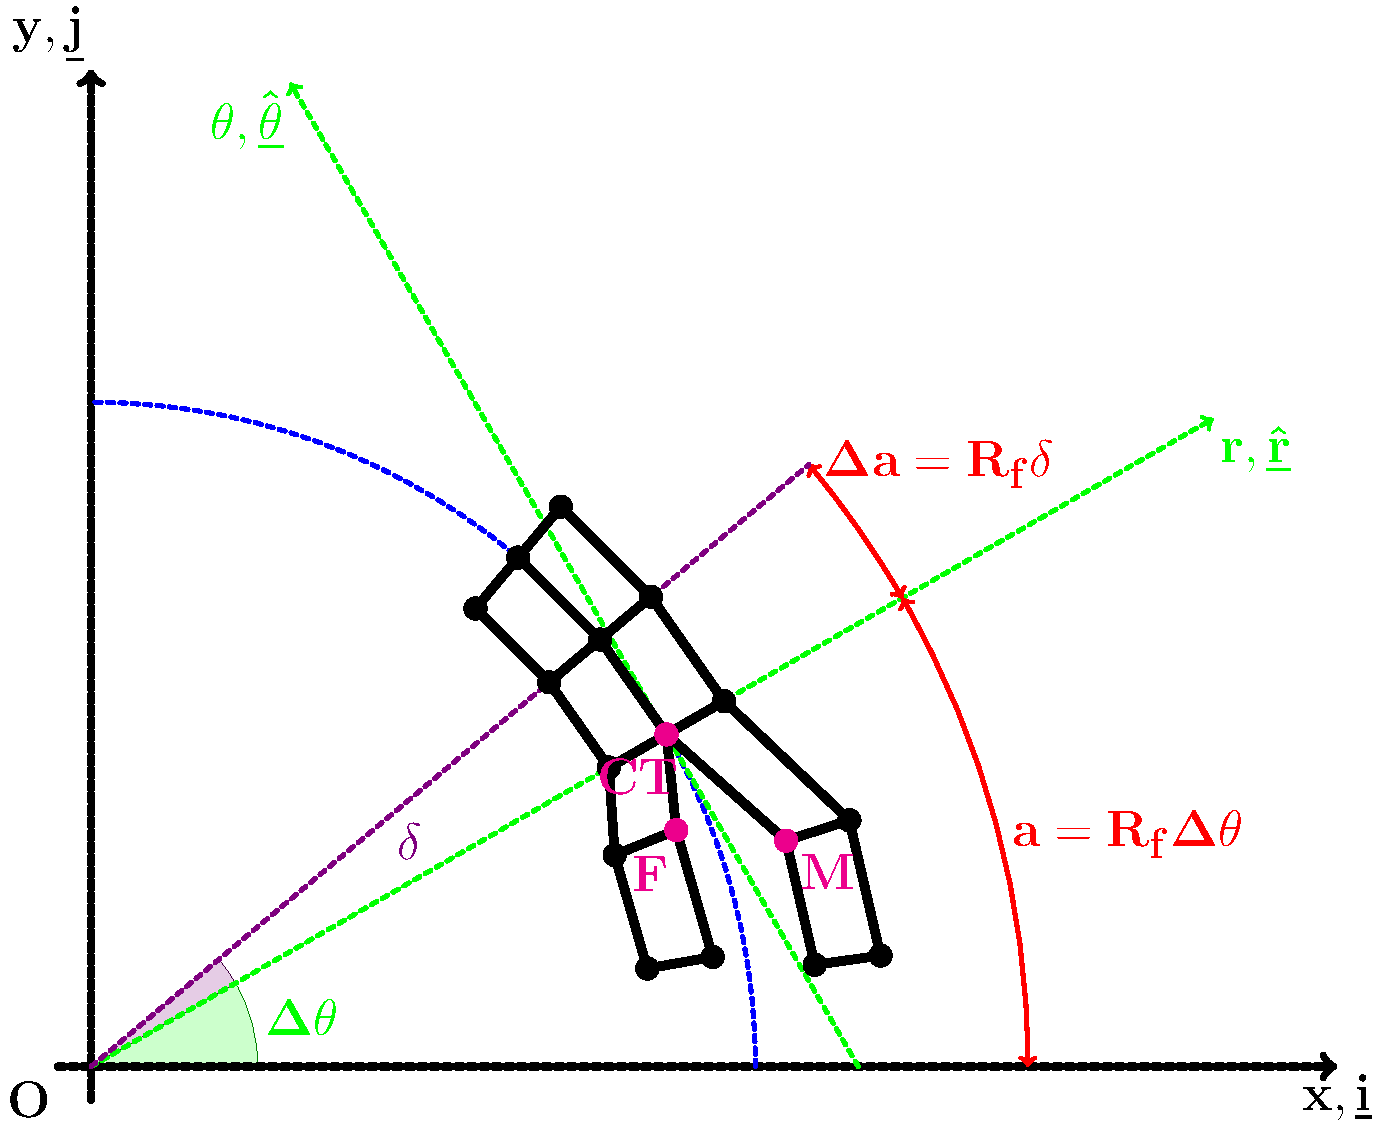
\includegraphics[width=\textwidth]{VCCT-linear.pdf}
\caption{Schematic representation of the discretized crack tip geometry for  $1^{st}$ order quadrilateral elements.}
\end{figure}

\begin{equation}
\underline{\underline{R}}=\begin{bmatrix}
\cos\left(\Delta\theta\right) & \sin\left(\Delta\theta\right) \\
-\sin\left(\Delta\theta\right) & \cos\left(\Delta\theta\right)
\end{bmatrix}\qquad\underline{\underline{R}}^{-1}=\underline{\underline{R}}^{T}=\begin{bmatrix}
\cos\left(\Delta\theta\right) & -\sin\left(\Delta\theta\right) \\
\sin\left(\Delta\theta\right) & \cos\left(\Delta\theta\right)
\end{bmatrix}
\end{equation}

\begin{equation}
\begin{bmatrix}
r \\
\theta
\end{bmatrix}=\underline{\underline{R}}\begin{bmatrix}
x \\
y
\end{bmatrix}\qquad\begin{bmatrix}
x \\
y
\end{bmatrix}=\underline{\underline{R}}^{-1}\begin{bmatrix}
r \\
\theta
\end{bmatrix}
\end{equation}

\subsection{Calculation of displacements and reaction forces}

\begin{equation}
u_{x}=u_{x,M}-u_{x,F}\qquad u_{y}=u_{y,M}-u_{y,F}
\end{equation}

\begin{equation}
u_{r}=\cos\left(\Delta\theta\right) u_{x}+\sin\left(\Delta\theta\right) u_{y}\qquad u_{\theta}=-\sin\left(\Delta\theta\right) u_{x}+\cos\left(\Delta\theta\right) u_{y}
\end{equation}

\begin{equation}
F_{r}=\cos\left(\Delta\theta\right) F_{x,CT}+\sin\left(\Delta\theta\right) F_{y,CT}\qquad F_{\theta}=-\sin\left(\Delta\theta\right) F_{x,CT}+\cos\left(\Delta\theta\right) F_{y,CT}
\end{equation}

\begin{equation}
\begin{cases}
&\left(k_{e,M|11}+k_{e,M|33}\right)u_{x,MCT}+\left(k_{e,M|12}+k_{e,M|34}\right)u_{y,MCT}+\\&+k_{e,M|13}u_{x,M}+k_{e,M|14}u_{y,M}+\left(k_{M|17}+k_{M|35}\right)u_{N,MC|7}+\left(k_{M|18}+k_{M|36}\right)u_{N,MC|8}+\\&+\sum_{i=5}^{6}k_{M|1i}u_{N,MC|i}+\sum_{i=7}^{8}k_{M|3i}u_{N,MB|i}+k_{M|31}u_{x,NCOI}+k_{M|32}u_{y,NCOI}=0\\[10pt]
&\left(k_{e,M|21}+k_{e,M|43}\right)u_{x,MCT}+\left(k_{e,M|22}+k_{e,M|44}\right)u_{y,MCT}+\\&+k_{e,M|23}u_{x,M}+k_{e,M|24}u_{y,M}+\left(k_{M|27}+k_{M|45}\right)u_{N,MC|7}+\left(k_{M|28}+k_{M|46}\right)u_{N,MC|8}+\\&+\sum_{i=5}^{6}k_{M|2i}u_{N,MC|i}+\sum_{i=7}^{8}k_{M|4i}u_{N,MB|i}+k_{M|41}u_{x,NCOI}+k_{M|42}u_{y,NCOI}=0\\[10pt]
&\left(k_{e,F|77}+k_{e,F|55}\right)u_{x,FCT}+\left(k_{e,F|78}+k_{e,F|56}\right)u_{y,FCT}+\\&+k_{e,F|75}u_{x,F}+k_{e,F|76}u_{y,F}+\left(k_{F|71}+k_{F|53}\right)u_{N,FC|1}+\left(k_{F|72}+k_{F|54}\right)u_{N,FC|2}+\\&+\sum_{i=2}^{3}k_{F|7i}u_{N,FC|i}+\sum_{i=1}^{2}k_{F|5i}u_{N,FB|i}+k_{F|57}u_{x,NCOI}+k_{F|58}u_{y,NCOI}=0\\[10pt]
&\left(k_{e,F|87}+k_{e,F|65}\right)u_{x,FCT}+\left(k_{e,F|88}+k_{e,F|66}\right)u_{y,FCT}+\\&+k_{e,F|85}u_{x,F}+k_{e,F|86}u_{y,F}+\left(k_{F|81}+k_{F|63}\right)u_{N,FC|1}+\left(k_{F|82}+k_{F|64}\right)u_{N,FC|2}+\\&+\sum_{i=2}^{3}k_{F|8i}u_{N,FC|i}+\sum_{i=1}^{2}k_{F|6i}u_{N,FB|i}+k_{F|67}u_{x,NCOI}+k_{F|68}u_{y,NCOI}=0\\[10pt]
&u_{x,FCT}-u_{x,MCT}-u_{x,DUMMY}=0\\
&u_{y,FCT}-u_{y,MCT}-u_{y,DUMMY}=0\\[10pt]
&u_{x,DUMMY}=0\\
&u_{y,DUMMY}=0\\
\end{cases}
\end{equation}

\begin{equation}
\begin{cases}
&\left(k_{e,M|11}+k_{e,M|33}\right)u_{x,MCT}+\left(k_{e,M|12}+k_{e,M|34}\right)u_{y,MCT}+\\&+k_{e,M|13}u_{x,M}+k_{e,M|14}u_{y,M}+\left(k_{M|17}+k_{M|35}\right)u_{N,MC|7}+\left(k_{M|18}+k_{M|36}\right)u_{N,MC|8}+\\&+\sum_{i=5}^{6}k_{M|1i}u_{N,MC|i}+\sum_{i=7}^{8}k_{M|3i}u_{N,MB|i}+k_{M|31}u_{x,NCOI}+k_{M|32}u_{y,NCOI}=0\\[10pt]
&\left(k_{e,M|21}+k_{e,M|43}\right)u_{x,MCT}+\left(k_{e,M|22}+k_{e,M|44}\right)u_{y,MCT}+\\&+k_{e,M|23}u_{x,M}+k_{e,M|24}u_{y,M}+\left(k_{M|27}+k_{M|45}\right)u_{N,MC|7}+\left(k_{M|28}+k_{M|46}\right)u_{N,MC|8}+\\&+\sum_{i=5}^{6}k_{M|2i}u_{N,MC|i}+\sum_{i=7}^{8}k_{M|4i}u_{N,MB|i}+k_{M|41}u_{x,NCOI}+k_{M|42}u_{y,NCOI}=0\\[10pt]
&\left(k_{e,F|77}+k_{e,F|55}\right)u_{x,MCT}+\left(k_{e,F|78}+k_{e,F|56}\right)u_{y,MCT}+\\&+k_{e,F|75}u_{x,F}+k_{e,F|76}u_{y,F}+\left(k_{F|71}+k_{F|53}\right)u_{N,FC|1}+\left(k_{F|72}+k_{F|54}\right)u_{N,FC|2}+\\&+\sum_{i=2}^{3}k_{F|7i}u_{N,FC|i}+\sum_{i=1}^{2}k_{F|5i}u_{N,FB|i}+k_{F|57}u_{x,NCOI}+k_{F|58}u_{y,NCOI}=0\\[10pt]
&\left(k_{e,F|87}+k_{e,F|65}\right)u_{x,MCT}+\left(k_{e,F|88}+k_{e,F|66}\right)u_{y,MCT}+\\&+k_{e,F|85}u_{x,F}+k_{e,F|86}u_{y,F}+\left(k_{F|81}+k_{F|63}\right)u_{N,FC|1}+\left(k_{F|82}+k_{F|64}\right)u_{N,FC|2}+\\&+\sum_{i=2}^{3}k_{F|8i}u_{N,FC|i}+\sum_{i=1}^{2}k_{F|6i}u_{N,FB|i}+k_{F|67}u_{x,NCOI}+k_{F|68}u_{y,NCOI}=0\\[10pt]
&u_{x,FCT}=u_{x,MCT}\\
&u_{y,FCT}=u_{y,MCT}\\[10pt]
&R_{x,DUMMY}=R_{x,FCT}=-R_{x,MCT}=F_{x,CT}\\
&R_{y,DUMMY}=R_{y,FCT}=-R_{y,MCT}=F_{y,CT}\\
\end{cases}
\end{equation}

\begin{equation}
\footnotesize
\begin{cases}
&\left(k_{e,M|11}+k_{e,M|33}+k_{e,F|77}+k_{e,F|55}\right)u_{x,MCT}+\left(k_{e,M|12}+k_{e,M|34}+k_{e,F|78}+k_{e,F|56}\right)u_{y,MCT}+\\&+k_{e,M|13}u_{x,M}+k_{e,M|14}u_{y,M}+k_{e,F|75}u_{x,F}+k_{e,F|76}u_{y,F}+\\&+\left(k_{M|31}+k_{F|57}\right)u_{x,NCOI}+\left(k_{M|32}+k_{F|58}\right)u_{y,NCOI}+\\&+\left(k_{M|17}+k_{M|35}\right)u_{N,MC|7}+\left(k_{M|18}+k_{M|36}\right)u_{N,MC|8}+\left(k_{F|71}+k_{F|53}\right)u_{N,FC|1}+\left(k_{F|72}+k_{F|54}\right)u_{N,FC|2}+\\&+\sum_{i=5}^{6}k_{M|1i}u_{N,MC|i}+\sum_{i=7}^{8}k_{M|3i}u_{N,MB|i}+\sum_{i=2}^{3}k_{F|7i}u_{N,FC|i}+\sum_{i=1}^{2}k_{F|5i}u_{N,FB|i}=0\\[10pt]
&\left(k_{e,M|21}+k_{e,M|43}+k_{e,F|87}+k_{e,F|65}\right)u_{x,MCT}+\left(k_{e,M|22}+k_{e,M|44}+k_{e,F|88}+k_{e,F|66}\right)u_{y,MCT}+\\&+k_{e,M|23}u_{x,M}+k_{e,M|24}u_{y,M}+k_{e,F|85}u_{x,F}+k_{e,F|86}u_{y,F}+\\&+\left(k_{M|41}+k_{F|67}\right)u_{x,NCOI}+\left(k_{M|42}+k_{F|68}\right)u_{y,NCOI}+\\&+\left(k_{M|27}+k_{M|45}\right)u_{N,MC|7}+\left(k_{M|28}+k_{M|46}\right)u_{N,MC|8}+\left(k_{F|81}+k_{F|63}\right)u_{N,FC|1}+\left(k_{F|82}+k_{F|64}\right)u_{N,FC|2}+\\&+\sum_{i=2}^{3}k_{F|8i}u_{N,FC|i}+\sum_{i=1}^{2}k_{F|6i}u_{N,FB|i}+\sum_{i=5}^{6}k_{M|2i}u_{N,MC|i}+\sum_{i=7}^{8}k_{M|4i}u_{N,MB|i}=0\\[10pt]
&u_{x,FCT}=u_{x,MCT}\\
&u_{y,FCT}=u_{y,MCT}\\[10pt]
&R_{x,DUMMY}=R_{x,FCT}=-R_{x,MCT}=F_{x,CT}\\
&R_{y,DUMMY}=R_{y,FCT}=-R_{y,MCT}=F_{y,CT}\\
\end{cases}
\end{equation}

\begin{equation}
\scriptsize
\begin{cases}
&u_{y,MCT}=-\frac{k_{e,M|11}+k_{e,M|33}+k_{e,F|77}+k_{e,F|55}}{k_{e,M|12}+k_{e,M|34}+k_{e,F|78}+k_{e,F|56}}u_{x,MCT}+\\
&-\frac{k_{e,M|13}u_{x,M}+k_{e,M|14}u_{y,M}+k_{e,F|75}u_{x,F}+k_{e,F|76}u_{y,F}}{k_{e,M|12}+k_{e,M|34}+k_{e,F|78}+k_{e,F|56}}+\\
&-\frac{\left(k_{M|31}+k_{F|57}\right)u_{x,NCOI}+\left(k_{M|32}+k_{F|58}\right)u_{y,NCOI}}{k_{e,M|12}+k_{e,M|34}+k_{e,F|78}+k_{e,F|56}}+\\
&-\frac{\left(k_{M|17}+k_{M|35}\right)u_{N,MC|7}+\left(k_{M|18}+k_{M|36}\right)u_{N,MC|8}+\left(k_{F|71}+k_{F|53}\right)u_{N,FC|1}+\left(k_{F|72}+k_{F|54}\right)u_{N,FC|2}}{k_{e,M|12}+k_{e,M|34}+k_{e,F|78}+k_{e,F|56}}+\\
&-\frac{\sum_{i=5}^{6}k_{M|1i}u_{N,MC|i}+\sum_{i=7}^{8}k_{M|3i}u_{N,MB|i}+\sum_{i=2}^{3}k_{F|7i}u_{N,FC|i}+\sum_{i=1}^{2}k_{F|5i}u_{N,FB|i}}{k_{e,M|12}+k_{e,M|34}+k_{e,F|78}+k_{e,F|56}}\\[10pt]

&\left[\left(k_{e,M|21}+k_{e,M|43}+k_{e,F|87}+k_{e,F|65}\right)+\frac{k_{e,M|11}+k_{e,M|33}+k_{e,F|77}+k_{e,F|55}}{k_{e,M|12}+k_{e,M|34}+k_{e,F|78}+k_{e,F|56}}\left(k_{e,M|22}+k_{e,M|44}+k_{e,F|88}+k_{e,F|66}\right)\right]u_{x,MCT}+\\
&+\left(k_{e,M|23}-\frac{k_{e,M|22}+k_{e,M|44}+k_{e,F|88}+k_{e,F|66}}{k_{e,M|12}+k_{e,M|34}+k_{e,F|78}+k_{e,F|56}}k_{e,M|13}\right)u_{x,M}+\\
&+\left(k_{e,M|24}-\frac{k_{e,M|22}+k_{e,M|44}+k_{e,F|88}+k_{e,F|66}}{k_{e,M|12}+k_{e,M|34}+k_{e,F|78}+k_{e,F|56}}k_{e,M|14}\right)u_{y,M}+\\
&+\left(k_{e,F|85}-\frac{k_{e,M|22}+k_{e,M|44}+k_{e,F|88}+k_{e,F|66}}{k_{e,M|12}+k_{e,M|34}+k_{e,F|78}+k_{e,F|56}}k_{e,M|75}\right)u_{x,F}+\\
&+\left(k_{e,F|86}-\frac{k_{e,M|22}+k_{e,M|44}+k_{e,F|88}+k_{e,F|66}}{k_{e,M|12}+k_{e,M|34}+k_{e,F|78}+k_{e,F|56}}k_{e,M|76}\right)u_{y,F}+\\
&+\left[\left(k_{M|41}+k_{F|67}\right)-\frac{k_{e,M|22}+k_{e,M|44}+k_{e,F|88}+k_{e,F|66}}{k_{e,M|12}+k_{e,M|34}+k_{e,F|78}+k_{e,F|56}}\left(k_{M|31}+k_{F|57}\right)\right]u_{x,NCOI}+\\
&+\left[\left(k_{M|42}+k_{F|68}\right)-\frac{k_{e,M|22}+k_{e,M|44}+k_{e,F|88}+k_{e,F|66}}{k_{e,M|12}+k_{e,M|34}+k_{e,F|78}+k_{e,F|56}}\left(k_{M|32}+k_{F|58}\right)\right]u_{y,NCOI}+\\
&+\left(k_{M|27}+k_{M|45}\right)u_{N,MC|7}+\left(k_{M|28}+k_{M|46}\right)u_{N,MC|8}+\left(k_{F|81}+k_{F|63}\right)u_{N,FC|1}+\left(k_{F|82}+k_{F|64}\right)u_{N,FC|2}+\\
&-\frac{k_{e,M|22}+k_{e,M|44}+k_{e,F|88}+k_{e,F|66}}{k_{e,M|12}+k_{e,M|34}+k_{e,F|78}+k_{e,F|56}}\left[\left(k_{M|17}+k_{M|35}\right)u_{N,MC|7}+\left(k_{M|18}+k_{M|36}\right)u_{N,MC|8}\right]+\\&
-\frac{k_{e,M|22}+k_{e,M|44}+k_{e,F|88}+k_{e,F|66}}{k_{e,M|12}+k_{e,M|34}+k_{e,F|78}+k_{e,F|56}}\left[\left(k_{F|71}+k_{F|53}\right)u_{N,FC|1}+\left(k_{F|72}+k_{F|54}\right)u_{N,FC|2}\right]\\
&+\sum_{i=2}^{3}k_{F|8i}u_{N,FC|i}+\sum_{i=1}^{2}k_{F|6i}u_{N,FB|i}+\sum_{i=5}^{6}k_{M|2i}u_{N,MC|i}+\sum_{i=7}^{8}k_{M|4i}u_{N,MB|i}+\\
&-\frac{\sum_{i=5}^{6}k_{M|1i}u_{N,MC|i}+\sum_{i=7}^{8}k_{M|3i}u_{N,MB|i}+\sum_{i=2}^{3}k_{F|7i}u_{N,FC|i}+\sum_{i=1}^{2}k_{F|5i}u_{N,FB|i}}{k_{e,M|12}+k_{e,M|34}+k_{e,F|78}+k_{e,F|56}}=0\\[10pt]

&u_{x,FCT}=u_{x,MCT}\\
&u_{y,FCT}=u_{y,MCT}\\[10pt]
&R_{x,DUMMY}=R_{x,FCT}=-R_{x,MCT}=F_{x,CT}\\
&R_{y,DUMMY}=R_{y,FCT}=-R_{y,MCT}=F_{y,CT}\\
\end{cases}
\end{equation}

\begin{equation}
\scriptsize
\begin{cases}
&u_{y,MCT}=-\frac{k_{e,M|11}+k_{e,M|33}+k_{e,F|77}+k_{e,F|55}}{k_{e,M|12}+k_{e,M|34}+k_{e,F|78}+k_{e,F|56}}u_{x,MCT}+\\
&-\frac{k_{e,M|13}u_{x,M}+k_{e,M|14}u_{y,M}+k_{e,F|75}u_{x,F}+k_{e,F|76}u_{y,F}}{k_{e,M|12}+k_{e,M|34}+k_{e,F|78}+k_{e,F|56}}+\\
&-\frac{\left(k_{M|31}+k_{F|57}\right)u_{x,NCOI}+\left(k_{M|32}+k_{F|58}\right)u_{y,NCOI}}{k_{e,M|12}+k_{e,M|34}+k_{e,F|78}+k_{e,F|56}}+\\
&-\frac{\left(k_{M|17}+k_{M|35}\right)u_{N,MC|7}+\left(k_{M|18}+k_{M|36}\right)u_{N,MC|8}+\left(k_{F|71}+k_{F|53}\right)u_{N,FC|1}+\left(k_{F|72}+k_{F|54}\right)u_{N,FC|2}}{k_{e,M|12}+k_{e,M|34}+k_{e,F|78}+k_{e,F|56}}+\\
&-\frac{\sum_{i=5}^{6}k_{M|1i}u_{N,MC|i}+\sum_{i=7}^{8}k_{M|3i}u_{N,MB|i}+\sum_{i=2}^{3}k_{F|7i}u_{N,FC|i}+\sum_{i=1}^{2}k_{F|5i}u_{N,FB|i}}{k_{e,M|12}+k_{e,M|34}+k_{e,F|78}+k_{e,F|56}}\\[10pt]

&\left[\left(k_{e,M|21}+k_{e,M|43}+k_{e,F|87}+k_{e,F|65}\right)+\frac{k_{e,M|11}+k_{e,M|33}+k_{e,F|77}+k_{e,F|55}}{k_{e,M|12}+k_{e,M|34}+k_{e,F|78}+k_{e,F|56}}\left(k_{e,M|22}+k_{e,M|44}+k_{e,F|88}+k_{e,F|66}\right)\right]u_{x,MCT}+\\
&+\left(k_{e,M|23}-\frac{k_{e,M|22}+k_{e,M|44}+k_{e,F|88}+k_{e,F|66}}{k_{e,M|12}+k_{e,M|34}+k_{e,F|78}+k_{e,F|56}}k_{e,M|13}\right)u_{x}+\\
&+\left(k_{e,M|24}-\frac{k_{e,M|22}+k_{e,M|44}+k_{e,F|88}+k_{e,F|66}}{k_{e,M|12}+k_{e,M|34}+k_{e,F|78}+k_{e,F|56}}k_{e,M|14}\right)u_{y}+\\
&+\left(k_{e,M|23}+k_{e,F|85}-\frac{k_{e,M|22}+k_{e,M|44}+k_{e,F|88}+k_{e,F|66}}{k_{e,M|12}+k_{e,M|34}+k_{e,F|78}+k_{e,F|56}}\left(k_{e,M|13}+k_{e,M|75}\right)\right)\cancelto{\approx 0}{u_{x,F}}+\\
&+\left(k_{e,M|24}+k_{e,F|86}-\frac{k_{e,M|22}+k_{e,M|44}+k_{e,F|88}+k_{e,F|66}}{k_{e,M|12}+k_{e,M|34}+k_{e,F|78}+k_{e,F|56}}\left(k_{e,M|14}+k_{e,M|76}\right)\right)\cancelto{\approx 0}{u_{y,F}}+\\
&+\left[\left(k_{M|41}+k_{F|67}\right)-\frac{k_{e,M|22}+k_{e,M|44}+k_{e,F|88}+k_{e,F|66}}{k_{e,M|12}+k_{e,M|34}+k_{e,F|78}+k_{e,F|56}}\left(k_{M|31}+k_{F|57}\right)\right]u_{x,NCOI}+\\
&+\left[\left(k_{M|42}+k_{F|68}\right)-\frac{k_{e,M|22}+k_{e,M|44}+k_{e,F|88}+k_{e,F|66}}{k_{e,M|12}+k_{e,M|34}+k_{e,F|78}+k_{e,F|56}}\left(k_{M|32}+k_{F|58}\right)\right]u_{y,NCOI}+\\
&+\left(k_{M|27}+k_{M|45}\right)u_{N,MC|7}+\left(k_{M|28}+k_{M|46}\right)u_{N,MC|8}+\left(k_{F|81}+k_{F|63}\right)u_{N,FC|1}+\left(k_{F|82}+k_{F|64}\right)u_{N,FC|2}+\\
&-\frac{k_{e,M|22}+k_{e,M|44}+k_{e,F|88}+k_{e,F|66}}{k_{e,M|12}+k_{e,M|34}+k_{e,F|78}+k_{e,F|56}}\left[\left(k_{M|17}+k_{M|35}\right)u_{N,MC|7}+\left(k_{M|18}+k_{M|36}\right)u_{N,MC|8}\right]+\\&
-\frac{k_{e,M|22}+k_{e,M|44}+k_{e,F|88}+k_{e,F|66}}{k_{e,M|12}+k_{e,M|34}+k_{e,F|78}+k_{e,F|56}}\left[\left(k_{F|71}+k_{F|53}\right)u_{N,FC|1}+\left(k_{F|72}+k_{F|54}\right)u_{N,FC|2}\right]\\
&+\sum_{i=2}^{3}k_{F|8i}u_{N,FC|i}+\sum_{i=1}^{2}k_{F|6i}u_{N,FB|i}+\sum_{i=5}^{6}k_{M|2i}u_{N,MC|i}+\sum_{i=7}^{8}k_{M|4i}u_{N,MB|i}+\\
&-\frac{\sum_{i=5}^{6}k_{M|1i}u_{N,MC|i}+\sum_{i=7}^{8}k_{M|3i}u_{N,MB|i}+\sum_{i=2}^{3}k_{F|7i}u_{N,FC|i}+\sum_{i=1}^{2}k_{F|5i}u_{N,FB|i}}{k_{e,M|12}+k_{e,M|34}+k_{e,F|78}+k_{e,F|56}}=0\\[10pt]

&u_{x,FCT}=u_{x,MCT}\\
&u_{y,FCT}=u_{y,MCT}\\[10pt]
F_{x,CT}&=R_{x,FCT}=\\&=\left(k_{e,F|77}+k_{e,F|55}\right)u_{x,FCT}+\left(k_{e,F|78}+k_{e,F|56}\right)u_{y,FCT}+\\
&+k_{e,F|75}\cancelto{\approx 0}{u_{x,F}}+k_{e,F|76}\cancelto{\approx 0}{u_{y,F}}+\\
&+\sum_{i=1}^{4}k_{e,F|7i}u_{N,FC|i}+\sum_{i=1,i\neq\left(5,6\right)}^{8}k_{e,F|5i}u_{N,FB|i}\\
F_{y,CT}&=R_{y,FCT}=\\&=\left(k_{e,F|87}+k_{e,F|65}\right)u_{x,FCT}+\left(k_{e,F|88}+k_{e,F|66}\right)u_{y,FCT}+\\
&+k_{e,F|85}\cancelto{\approx 0}{u_{x,F}}+k_{e,F|86}\cancelto{\approx 0}{u_{y,F}}+\\
&+\sum_{i=1}^{4}k_{e,F|8i}u_{N,FC|i}+\sum_{i=1,i\neq\left(5,6\right)}^{8}k_{e,F|6i}u_{N,FB|i}\\
\end{cases}
\end{equation}

\begin{equation}
\begin{cases}
F_{x,CT}&=\left(k_{e,F|77}+k_{e,F|55}\right)u_{x,MCT}+\left(k_{e,F|78}+k_{e,F|56}\right)u_{y,MCT}+\\
&+\sum_{i=1}^{4}k_{e,F|7i}u_{N,FC|i}+\sum_{i=1,i\neq\left(5,6\right)}^{8}k_{e,F|5i}u_{N,FB|i}\\
F_{y,CT}&=\left(k_{e,F|87}+k_{e,F|65}\right)u_{x,MCT}+\left(k_{e,F|88}+k_{e,F|66}\right)u_{y,MCT}+\\
&+\sum_{i=1}^{4}k_{e,F|8i}u_{N,FC|i}+\sum_{i=1,i\neq\left(5,6\right)}^{8}k_{e,F|6i}u_{N,FB|i}\\
\end{cases}
\end{equation}

\begin{equation}
\begin{cases}
F_{x,CT}&= K_{xx}u_{x}+K_{xy}u_{y}+\\
&+\sum_{i=1}^{4}K_{FC,x|i}u_{N,FC|i}+\sum_{i=1,i\neq\left(3,4,5,6\right)}^{8}K_{FB,x|i}u_{N,FB|i}+\\
&+\sum_{i=5}^{8}K_{FC,x|i}u_{N,MC|i}+\sum_{i=7}^{8}K_{MB,x|i}u_{N,FB|i}\\
F_{y,CT}&= K_{yx}u_{x}+K_{yy}u_{y}+\\
&+\sum_{i=1}^{4}K_{FC,y|i}u_{N,FC|i}+\sum_{i=1,i\neq\left(3,4,5,6\right)}^{8}K_{FB,y|i}u_{N,FB|i}+\\
&+\sum_{i=5}^{8}K_{FC,y|i}u_{N,MC|i}+\sum_{i=7}^{8}K_{MB,y|i}u_{N,FB|i}\\
\end{cases}
\end{equation}

\begin{equation}
\begin{cases}
F_{x,CT}&= K_{xx}u_{x}+K_{xy}u_{y}+\widetilde{F}_{x}\\
F_{y,CT}&= K_{yx}u_{x}+K_{yy}u_{y}+\widetilde{F}_{y}\\
\end{cases}
\end{equation}

\subsection{Calculation of energy release rates}

\begin{equation}
\begin{split}
G_{I,r\theta} = &\frac{1}{2}\frac{F_{r}u_{r}}{R_{f}\delta}=\\
= &\frac{1}{2R_{f}\delta}\left(\cos\left(\Delta\theta\right) F_{x}+\sin\left(\Delta\theta\right)F_{y}\right)\left(\cos\left(\Delta\theta\right) u_{x}+\sin\left(\Delta\theta\right) u_{y}\right)=\\
= &\frac{1}{2R_{f}\delta}\left(\cos^{2}\left(\Delta\theta\right) F_{x}u_{x}+\left(F_{x}u_{y}+F_{y}u_{x}\right)\cos\left(\Delta\theta\right)\sin\left(\Delta\theta\right)+\sin^{2}\left(\Delta\theta\right)F_{y}u_{y}\right)\\
\end{split}
\end{equation}

\begin{equation}
\begin{split}
G_{II,r\theta} = &\frac{1}{2}\frac{F_{\theta}u_{\theta}}{R_{f}\delta}=\\
= &\frac{1}{2R_{f}\delta}\left(-\sin\left(\Delta\theta\right) F_{x}+\cos\left(\Delta\theta\right)F_{y}\right)\left(-\sin\left(\Delta\theta\right) u_{x}+\cos\left(\Delta\theta\right) u_{y}\right)=\\
= &\frac{1}{2R_{f}\delta}\left(\sin^{2}\left(\Delta\theta\right) F_{x}u_{x}-\left(F_{x}u_{y}+F_{y}u_{x}\right)\cos\left(\Delta\theta\right)\sin\left(\Delta\theta\right)+\cos^{2}\left(\Delta\theta\right)F_{y}u_{y}\right)\\
\end{split}
\end{equation}

\begin{equation}
\begin{split}
G_{TOT,r\theta} = &G_{I,r\theta} + G_{II,r\theta}=\\
= &\frac{1}{2R_{f}\delta}\left(\cos^{2}\left(\Delta\theta\right) F_{x}u_{x}+\left(F_{x}u_{y}+F_{y}u_{x}\right)\cos\left(\Delta\theta\right)\sin\left(\Delta\theta\right)+\sin^{2}\left(\Delta\theta\right)F_{y}u_{y}\right)+\\
&+ \frac{1}{2R_{f}\delta}\left(\sin^{2}\left(\Delta\theta\right) F_{x}u_{x}-\left(F_{x}u_{y}+F_{y}u_{x}\right)\cos\left(\Delta\theta\right)\sin\left(\Delta\theta\right)+\cos^{2}\left(\Delta\theta\right)F_{y}u_{y}\right)=\\
=&\frac{1}{2R_{f}\delta}\left(\cancelto{1}{\left(\cos^{2}\left(\Delta\theta\right)+\sin^{2}\left(\Delta\theta\right)\right)}F_{x}u_{x}\right)+\\
&+\frac{1}{2R_{f}\delta}\left(\cancelto{0}{\left(\left(F_{x}u_{y}+F_{y}u_{x}\right)-\left(F_{x}u_{y}+F_{y}u_{x}\right)\right)}\cos\left(\Delta\theta\right)\sin\left(\Delta\theta\right)\right)+\\
&+\frac{1}{2R_{f}\delta}\left(\cancelto{1}{\left(\cos^{2}\left(\Delta\theta\right)+\sin^{2}\left(\Delta\theta\right)\right)}F_{y}u_{y}\right)=\\
=&\frac{1}{2}\frac{F_{x}u_{x}}{R_{f}\delta}+\frac{1}{2}\frac{F_{y}u_{y}}{R_{f}\delta}=\\
=&\widetilde{G}_{I,xy} + \widetilde{G}_{II,xy}=\widetilde{G}_{TOT,xy}
\end{split}
\end{equation}

\begin{equation}
\begin{split}
G_{I,r\theta} =&\frac{1}{2R_{f}\delta}\left(\cos^{2}\left(\Delta\theta\right) F_{x}u_{x}+\left(F_{x}u_{y}+F_{y}u_{x}\right)\cos\left(\Delta\theta\right)\sin\left(\Delta\theta\right)+\sin^{2}\left(\Delta\theta\right)F_{y}u_{y}\right)=\\
=&\cos^{2}\left(\Delta\theta\right)\frac{ F_{x}u_{x}}{2R_{f}\delta}+\left(\frac{F_{x}u_{y}}{2R_{f}\delta}+\frac{F_{y}u_{x}}{2R_{f}\delta}\right)\cos\left(\Delta\theta\right)\sin\left(\Delta\theta\right)+\sin^{2}\left(\Delta\theta\right)\frac{F_{y}u_{y}}{2R_{f}\delta}=\\
=&\cos^{2}\left(\Delta\theta\right)\widetilde{G}_{I,xy}+\left(\widetilde{G}_{I,xy}\frac{u_{y}}{u_{x}}+\widetilde{G}_{II,xy}\frac{u_{x}}{u_{y}}\right)\cos\left(\Delta\theta\right)\sin\left(\Delta\theta\right)+\sin^{2}\left(\Delta\theta\right)\widetilde{G}_{II,xy}
\end{split}
\end{equation}

\begin{equation}
\begin{split}
G_{II,r\theta} =&\frac{1}{2R_{f}\delta}\left(\sin^{2}\left(\Delta\theta\right) F_{x}u_{x}-\left(F_{x}u_{y}+F_{y}u_{x}\right)\cos\left(\Delta\theta\right)\sin\left(\Delta\theta\right)+\cos^{2}\left(\Delta\theta\right)F_{y}u_{y}\right)=\\
=&\sin^{2}\left(\Delta\theta\right)\frac{ F_{x}u_{x}}{2R_{f}\delta}-\left(\frac{F_{x}u_{y}}{2R_{f}\delta}+\frac{F_{y}u_{x}}{2R_{f}\delta}\right)\cos\left(\Delta\theta\right)\sin\left(\Delta\theta\right)+\cos^{2}\left(\Delta\theta\right)\frac{F_{y}u_{y}}{2R_{f}\delta}=\\
=&\sin^{2}\left(\Delta\theta\right)\widetilde{G}_{I,xy}-\left(\widetilde{G}_{I,xy}\frac{u_{y}}{u_{x}}+\widetilde{G}_{II,xy}\frac{u_{x}}{u_{y}}\right)\cos\left(\Delta\theta\right)\sin\left(\Delta\theta\right)+\cos^{2}\left(\Delta\theta\right)\widetilde{G}_{II,xy}
\end{split}
\end{equation}

\subsection{Sensitivity analysis of the FEM solution}

\begin{equation}
\begin{cases}
F_{x,CT}&= K_{xx}u_{x}+K_{xy}u_{y}+\widetilde{F}_{x}\\
F_{y,CT}&= K_{yx}u_{x}+K_{yy}u_{y}+\widetilde{F}_{y}\\
\end{cases}
\end{equation}

\begin{equation}
\begin{split}
G_{I,r\theta} \sim&\frac{1}{2R_{f}\delta}\cos^{2}\left(\Delta\theta\right) \left(K_{xx}u^{2}_{x}+K_{xy}u_{y}u_{x}+\widetilde{F}_{x}u_{x}\right)+\\
&+\frac{1}{2R_{f}\delta}\cos\left(\Delta\theta\right)\sin\left(\Delta\theta\right)\left(K_{xx}u_{x}u_{y}+K_{xy}u^{2}_{y}+\widetilde{F}_{x}u_{y}\right)+\\
&+\frac{1}{2R_{f}\delta}\cos\left(\Delta\theta\right)\sin\left(\Delta\theta\right)\left(K_{yx}u^{2}_{x}+K_{yy}u_{y}u_{x}+\widetilde{F}_{y}u_{x}\right)+\\
&+\frac{1}{2R_{f}\delta}\sin^{2}\left(\Delta\theta\right)\left(K_{yx}u_{y}u_{x}+K_{yy}u^{2}_{y}+\widetilde{F}_{y}\right)
\end{split}
\end{equation}

\begin{equation}
\begin{split}
G_{II,r\theta} \sim&\frac{1}{2R_{f}\delta}\sin^{2}\left(\Delta\theta\right) k_{x}u^{2}_{x}\left(\Delta\theta\right)+\\
&-\frac{1}{2R_{f}\delta}\left(k_{x}+k_{y}\right)u_{x}\left(\Delta\theta\right)u_{y}\left(\Delta\theta\right)\cos\left(\Delta\theta\right)\sin\left(\Delta\theta\right)+\\
&+\frac{1}{2R_{f}\delta}\cos^{2}\left(\Delta\theta\right)k_{y}u^{2}_{y}\left(\Delta\theta\right)
\end{split}
\end{equation}

\begin{equation}
G_{TOT,r\theta} \sim\frac{1}{2R_{f}\delta}\left( k_{x}u^{2}_{x}\left(\Delta\theta\right)+ k_{y}u^{2}_{y}\left(\Delta\theta\right)\right)
\end{equation}

\begin{equation}
\begin{split}
\frac{\partial G_{I,r\theta}}{\partial\Delta\theta} \sim&\frac{1}{R_{f}\delta}\cos^{2}\left(\Delta\theta\right) k_{x}u_{x}\left(\Delta\theta\right)\frac{\partial u_{x}\left(\Delta\theta\right)}{\partial\Delta\theta}+\\
&+\frac{1}{2R_{f}\delta}\left(k_{x}+k_{y}\right)\left(\frac{\partial u_{x}\left(\Delta\theta\right)}{\partial\Delta\theta}u_{y}\left(\Delta\theta\right)+u_{x}\left(\Delta\theta\right)\frac{\partial u_{y}\left(\Delta\theta\right)}{\partial\Delta\theta}\right)\cos\left(\Delta\theta\right)\sin\left(\Delta\theta\right)+\\
&+\frac{1}{R_{f}\delta}\sin^{2}\left(\Delta\theta\right)k_{y}u_{y}\left(\Delta\theta\right)\frac{\partial u_{y}\left(\Delta\theta\right)}{\partial\Delta\theta}+\\
&+\frac{1}{2R_{f}\delta}\left(k_{y}u^{2}_{y}\left(\Delta\theta\right)- k_{x}u^{2}_{x}\left(\Delta\theta\right)\right)\sin\left(2\Delta\theta\right)+\\
&+\frac{1}{2R_{f}\delta}\left(k_{x}u_{x}\left(\Delta\theta\right)u_{y}\left(\Delta\theta\right)+k_{y}u_{y}\left(\Delta\theta\right)u_{x}\left(\Delta\theta\right)\right)\cos\left(2\Delta\theta\right)\\
\end{split}
\end{equation}

\begin{equation}
\begin{split}
\frac{\partial G_{II,r\theta}}{\partial\Delta\theta} \sim&\frac{1}{R_{f}\delta}\sin^{2}\left(\Delta\theta\right) k_{x}u_{x}\left(\Delta\theta\right)\frac{\partial u_{x}\left(\Delta\theta\right)}{\partial\Delta\theta}+\\
&-\frac{1}{2R_{f}\delta}\left(k_{x}+k_{y}\right)\left(\frac{\partial u_{x}\left(\Delta\theta\right)}{\partial\Delta\theta}u_{y}\left(\Delta\theta\right)+u_{x}\left(\Delta\theta\right)\frac{\partial u_{y}\left(\Delta\theta\right)}{\partial\Delta\theta}\right)\cos\left(\Delta\theta\right)\sin\left(\Delta\theta\right)+\\
&+\frac{1}{R_{f}\delta}\cos^{2}\left(\Delta\theta\right)k_{y}u_{y}\left(\Delta\theta\right)\frac{\partial u_{y}\left(\Delta\theta\right)}{\partial\Delta\theta}+\\
&+\frac{1}{2R_{f}\delta}\left(k_{x}u^{2}_{x}\left(\Delta\theta\right)- k_{y}u^{2}_{y}\left(\Delta\theta\right)\right)\sin\left(2\Delta\theta\right)+\\
&-\frac{1}{2R_{f}\delta}\left(k_{x}u_{x}\left(\Delta\theta\right)u_{y}\left(\Delta\theta\right)+k_{y}u_{y}\left(\Delta\theta\right)u_{x}\left(\Delta\theta\right)\right)\cos\left(2\Delta\theta\right)\\
\end{split}
\end{equation}

\begin{equation}
\frac{\partial G_{TOT,r\theta}}{\partial\Delta\theta} \sim\frac{1}{R_{f}\delta}\left( k_{x}u_{x}\left(\Delta\theta\right)\frac{\partial u_{x}\left(\Delta\theta\right)}{\partial\Delta\theta}+ k_{y}u_{y}\left(\Delta\theta\right)\frac{\partial u_{y}\left(\Delta\theta\right)}{\partial\Delta\theta}\right)
\end{equation}

\subsection{Discretization error}

\begin{equation}
u_{r}=\cos\left(\Delta\theta-\delta\right) u_{x}+\sin\left(\Delta\theta-\delta\right) u_{y}\qquad u_{\theta}=-\sin\left(\Delta\theta-\delta\right) u_{x}+\cos\left(\Delta\theta-\delta\right) u_{y}
\end{equation}

\begin{equation}
F_{r}=\cos\left(\Delta\theta\right) F_{x,CT}+\sin\left(\Delta\theta\right) F_{y,CT}\qquad F_{\theta}=-\sin\left(\Delta\theta\right) F_{x,CT}+\cos\left(\Delta\theta\right) F_{y,CT}
\end{equation}

\begin{equation}
\begin{split}
\widetilde{G}_{I,r\theta} = &\frac{1}{2}\frac{F_{r}u_{r}}{R_{f}\delta}=\\
= &\frac{1}{2R_{f}\delta}\left(\cos\left(\Delta\theta\right) F_{x}+\sin\left(\Delta\theta\right)F_{y}\right)\left(\cos\left(\Delta\theta-\delta\right) u_{x}+\sin\left(\Delta\theta-\delta\right) u_{y}\right)=\\
= &\frac{1}{2R_{f}\delta}\left(\cos\left(\Delta\theta\right) F_{x}+\sin\left(\Delta\theta\right)F_{y}\right)\left(\cos\left(\Delta\theta\right) u_{x}+\sin\left(\Delta\theta\right) u_{y}\right)\cos\left(\delta\right)+\\
&+\frac{1}{2R_{f}\delta}\left(\cos\left(\Delta\theta\right) F_{x}+\sin\left(\Delta\theta\right)F_{y}\right)\left(\sin\left(\Delta\theta\right) u_{x}-\cos\left(\Delta\theta\right) u_{y}\right)\sin\left(\delta\right)=\\
= &\frac{1}{2R_{f}\delta}\left(\cos^{2}\left(\Delta\theta\right) F_{x}u_{x}+\left(F_{x}u_{y}+F_{y}u_{x}\right)\cos\left(\Delta\theta\right)\sin\left(\Delta\theta\right)+\sin^{2}\left(\Delta\theta\right)F_{y}u_{y}\right)\cos\left(\delta\right)+\\
&+\frac{1}{2R_{f}\delta}\left(-\cos^{2}\left(\Delta\theta\right) F_{x}u_{y}+\left(F_{x}u_{x}-F_{y}u_{y}\right)\cos\left(\Delta\theta\right)\sin\left(\Delta\theta\right)+\sin^{2}\left(\Delta\theta\right)F_{y}u_{x}\right)\sin\left(\delta\right)=\\
= &G_{I,r\theta}\cos\left(\delta\right)+\\
&+\frac{1}{2R_{f}\delta}\left(-\cos^{2}\left(\Delta\theta\right) F_{x}u_{y}+\left(F_{x}u_{x}-F_{y}u_{y}\right)\cos\left(\Delta\theta\right)\sin\left(\Delta\theta\right)+\sin^{2}\left(\Delta\theta\right)F_{y}u_{x}\right)\sin\left(\delta\right)=\\
= &G_{I,r\theta}\cos\left(\delta\right)-\frac{1}{2R_{f}\delta}F_{r}u_{\theta}\sin{\delta}\\
\end{split}
\end{equation}

\begin{equation}
\begin{split}
\lim_{\delta\rightarrow 0}\widetilde{G}_{I,r\theta} = &\lim_{\delta\rightarrow 0}G_{I,r\theta}\cos\left(\delta\right)+\\
+\lim_{\delta\rightarrow 0}\frac{1}{2R_{f}\delta}&\left(-\cos^{2}\left(\Delta\theta\right) F_{x}u_{y}+\left(F_{x}u_{x}-F_{y}u_{y}\right)\cos\left(\Delta\theta\right)\sin\left(\Delta\theta\right)+\sin^{2}\left(\Delta\theta\right)F_{y}u_{x}\right)\sin\left(\delta\right)=\\
= &G_{I,r\theta}+\\
+\frac{1}{2R_{f}}&\left(-\cos^{2}\left(\Delta\theta\right) F_{x}u_{y}+\left(F_{x}u_{x}-F_{y}u_{y}\right)\cos\left(\Delta\theta\right)\sin\left(\Delta\theta\right)+\sin^{2}\left(\Delta\theta\right)F_{y}u_{x}\right)\lim_{\delta\rightarrow 0}\frac{\sin\left(\delta\right)}{\delta}=\\
= &G_{I,r\theta}+\frac{1}{2R_{f}}\left(-\cos^{2}\left(\Delta\theta\right) F_{x}u_{y}+\left(F_{x}u_{x}-F_{y}u_{y}\right)\cos\left(\Delta\theta\right)\sin\left(\Delta\theta\right)+\sin^{2}\left(\Delta\theta\right)F_{y}u_{x}\right)\\
= &G_{I,r\theta}-\frac{1}{2R_{f}}F_{r}u_{\theta}\\
\end{split}
\end{equation}

\begin{equation}
\begin{split}
\widetilde{G}_{II,r\theta} = &\frac{1}{2}\frac{F_{\theta}u_{\theta}}{R_{f}\delta}=\\
= &\frac{1}{2R_{f}\delta}\left(-\sin\left(\Delta\theta\right) F_{x}+\cos\left(\Delta\theta\right)F_{y}\right)\left(-\sin\left(\Delta\theta-\delta\right) u_{x}+\cos\left(\Delta\theta-\delta\right) u_{y}\right)=\\
= &\frac{1}{2R_{f}\delta}\left(\sin^{2}\left(\Delta\theta\right)\cos\left(\delta\right) F_{x}u_{x}-\left(F_{x}u_{y}+F_{y}u_{x}\right)\cos\left(\Delta\theta\right)\sin\left(\Delta\theta\right)\cos\left(\delta\right)+\cos^{2}\left(\Delta\theta\right)\cos\left(\delta\right)F_{y}u_{y}\right)+\\
+ &\frac{1}{2R_{f}\delta}\left(\left(F_{y}u_{y}-F_{x}u_{x}\right)\cos\left(\Delta\theta\right)\sin\left(\Delta\theta\right)\sin\left(\delta\right)+\cos^{2}\left(\Delta\theta\right)\sin\left(\delta\right)F_{y}u_{x}-\sin^{2}\left(\Delta\theta\right)\sin\left(\delta\right)F_{x}u_{y}\right)=\\
=&\frac{1}{2R_{f}\delta}\left(\sin^{2}\left(\Delta\theta\right) F_{x}u_{x}-\left(F_{x}u_{y}+F_{y}u_{x}\right)\cos\left(\Delta\theta\right)\sin\left(\Delta\theta\right)+\cos^{2}\left(\Delta\theta\right)F_{y}u_{y}\right)\cos\left(\delta\right)+\\
+ &\frac{1}{2R_{f}\delta}\left(\left(F_{y}u_{y}-F_{x}u_{x}\right)\cos\left(\Delta\theta\right)\sin\left(\Delta\theta\right)+\cos^{2}\left(\Delta\theta\right)F_{y}u_{x}-\sin^{2}\left(\Delta\theta\right)F_{x}u_{y}\right)\sin\left(\delta\right)=\\
=&G_{II,r\theta}\cos\left(\delta\right)+\\
+ &\frac{1}{2R_{f}\delta}\left(\left(F_{y}u_{y}-F_{x}u_{x}\right)\cos\left(\Delta\theta\right)\sin\left(\Delta\theta\right)+\cos^{2}\left(\Delta\theta\right)F_{y}u_{x}-\sin^{2}\left(\Delta\theta\right)F_{x}u_{y}\right)\sin\left(\delta\right)=\\
= &G_{II,r\theta}\cos\left(\delta\right)+\frac{1}{2R_{f}\delta}F_{\theta}u_{r}\sin{\delta}\\
\end{split}
\end{equation}

\begin{equation}
\begin{split}
\lim_{\delta\rightarrow 0}\widetilde{G}_{II,r\theta} = &\lim_{\delta\rightarrow 0}G_{II,r\theta}\cos\left(\delta\right)+\\
+\lim_{\delta\rightarrow 0}\frac{1}{2R_{f}\delta}&\left(\left(F_{y}u_{y}-F_{x}u_{x}\right)\cos\left(\Delta\theta\right)\sin\left(\Delta\theta\right)+\cos^{2}\left(\Delta\theta\right)F_{y}u_{x}-\sin^{2}\left(\Delta\theta\right)F_{x}u_{y}\right)\sin\left(\delta\right)=\\
= &G_{II,r\theta}+\\
+\frac{1}{2R_{f}\delta}&\left(\left(F_{y}u_{y}-F_{x}u_{x}\right)\cos\left(\Delta\theta\right)\sin\left(\Delta\theta\right)+\cos^{2}\left(\Delta\theta\right)F_{y}u_{x}-\sin^{2}\left(\Delta\theta\right)F_{x}u_{y}\right)\lim_{\delta\rightarrow 0}\frac{\sin\left(\delta\right)}{\delta}\\
= &G_{II,r\theta}+\frac{1}{2R_{f}\delta}\left(\left(F_{y}u_{y}-F_{x}u_{x}\right)\cos\left(\Delta\theta\right)\sin\left(\Delta\theta\right)+\cos^{2}\left(\Delta\theta\right)F_{y}u_{x}-\sin^{2}\left(\Delta\theta\right)F_{x}u_{y}\right)=\\
= &G_{II,r\theta}+\frac{1}{2R_{f}}F_{\theta}u_{r}\\
\end{split}
\end{equation}

\begin{equation}
\begin{split}
\widetilde{G}_{TOT,r\theta} &= \widetilde{G}_{I,r\theta} + \widetilde{G}_{II,r\theta}=\\
=&\left(G_{I,r\theta}+G_{II,r\theta}\right)\cos\left(\delta\right)+\\
+ &\frac{1}{2R_{f}\delta}\left(-\cos^{2}\left(\Delta\theta\right) F_{x}u_{y}+\left(F_{x}u_{x}-F_{y}u_{y}\right)\cos\left(\Delta\theta\right)\sin\left(\Delta\theta\right)+\sin^{2}\left(\Delta\theta\right)F_{y}u_{x}\right)\sin\left(\delta\right)+\\
+ &\frac{1}{2R_{f}\delta}\left(\left(F_{y}u_{y}-F_{x}u_{x}\right)\cos\left(\Delta\theta\right)\sin\left(\Delta\theta\right)+\cos^{2}\left(\Delta\theta\right)F_{y}u_{x}-\sin^{2}\left(\Delta\theta\right)F_{x}u_{y}\right)\sin\left(\delta\right)=\\
=&\left(G_{I,r\theta}+G_{II,r\theta}\right)\cos\left(\delta\right)+\frac{1}{2R_{f}\delta}\left(F_{y}u_{x}-F_{x}u_{y}\right)\sin\left(\delta\right)=\\
=&G_{TOT,r\theta}\cos\left(\delta\right)+\frac{1}{2R_{f}\delta}\left(F_{y}u_{x}-F_{x}u_{y}\right)\sin\left(\delta\right)=\\
=&G_{TOT,r\theta}\cos\left(\delta\right)+\frac{1}{2R_{f}\delta}\left(F_{\theta}u_{r}-F_{r}u_{\theta}\right)\sin\left(\delta\right)
\end{split}
\end{equation}

\begin{equation}
\begin{split}
\lim_{\delta\rightarrow 0}\widetilde{G}_{TOT,r\theta} = &\lim_{\delta\rightarrow 0}G_{TOT,r\theta}\cos\left(\delta\right)+\lim_{\delta\rightarrow 0}\frac{1}{2R_{f}\delta}\left(F_{y}u_{x}-F_{x}u_{y}\right)\sin\left(\delta\right)=\\
= &G_{TOT,r\theta}+\frac{1}{2R_{f}}\left(F_{y}u_{x}-F_{x}u_{y}\right)\lim_{\delta\rightarrow 0}\frac{\sin\left(\delta\right)}{\delta}-0\\
= &G_{TOT,r\theta}+\frac{1}{2R_{f}}\left(F_{y}u_{x}-F_{x}u_{y}\right)=\\
= &G_{TOT,r\theta}+\frac{1}{2R_{f}}\left(F_{\theta}u_{r}-F_{r}u_{\theta}\right)
\end{split}
\end{equation}

\subsection{Contact region}

\begin{equation}
u_{r}=0
\end{equation}

\begin{equation}
\cos\left(\Delta\theta\right) u_{x}+\sin\left(\Delta\theta\right) u_{y}=0
\end{equation}

\begin{equation}
u_{y}=-\frac{ u_{x}}{\tan\left(\Delta\theta\right)}
\end{equation}

\begin{equation}
\begin{split}
u_{\theta}=&-\sin\left(\Delta\theta\right) u_{x}-\frac{\cos^{2}\left(\Delta\theta\right)}{\sin\left(\Delta\theta\right)}u_{x}=\\
=&-\frac{u_{x}}{\sin\left(\Delta\theta\right)}
\end{split}
\end{equation}

\begin{equation}
F_{r}=\cos\left(\Delta\theta\right) F_{x,CT}+\sin\left(\Delta\theta\right) F_{y,CT}\qquad F_{\theta}=-\sin\left(\Delta\theta\right) F_{x,CT}+\cos\left(\Delta\theta\right) F_{y,CT}
\end{equation}

\begin{equation}
\begin{split}
G_{I,r\theta} = &\frac{1}{2}\frac{F_{r}u_{r}}{R_{f}\delta}=0
\end{split}
\end{equation}

\begin{equation}
\begin{split}
G_{II,r\theta} = &\frac{1}{2}\frac{F_{\theta}u_{\theta}}{R_{f}\delta}=\\
= &\frac{1}{2R_{f}\delta}\left(-\sin\left(\Delta\theta\right) F_{x}+\cos\left(\Delta\theta\right)F_{y}\right)\left(-\frac{u_{x}}{\sin\left(\Delta\theta\right)}\right)=\\
= &\frac{1}{2R_{f}\delta}\left( F_{x}u_{x}-\frac{F_{y}u_{x}}{\tan\left(\Delta\theta\right)}\right)\\
= &\frac{1}{2R_{f}\delta}\left( F_{x}-\frac{F_{y}}{\tan\left(\Delta\theta\right)}\right)u_{x}\\
\end{split}
\end{equation}

\clearpage

%------------------------------------------------------------------------------------------%
%                             VCCT 2nd order
%------------------------------------------------------------------------------------------%

\section{VCCT for second order quadrilateral elements}

\subsection{Definition of crack tip reference frame}

\begin{figure}[!h]
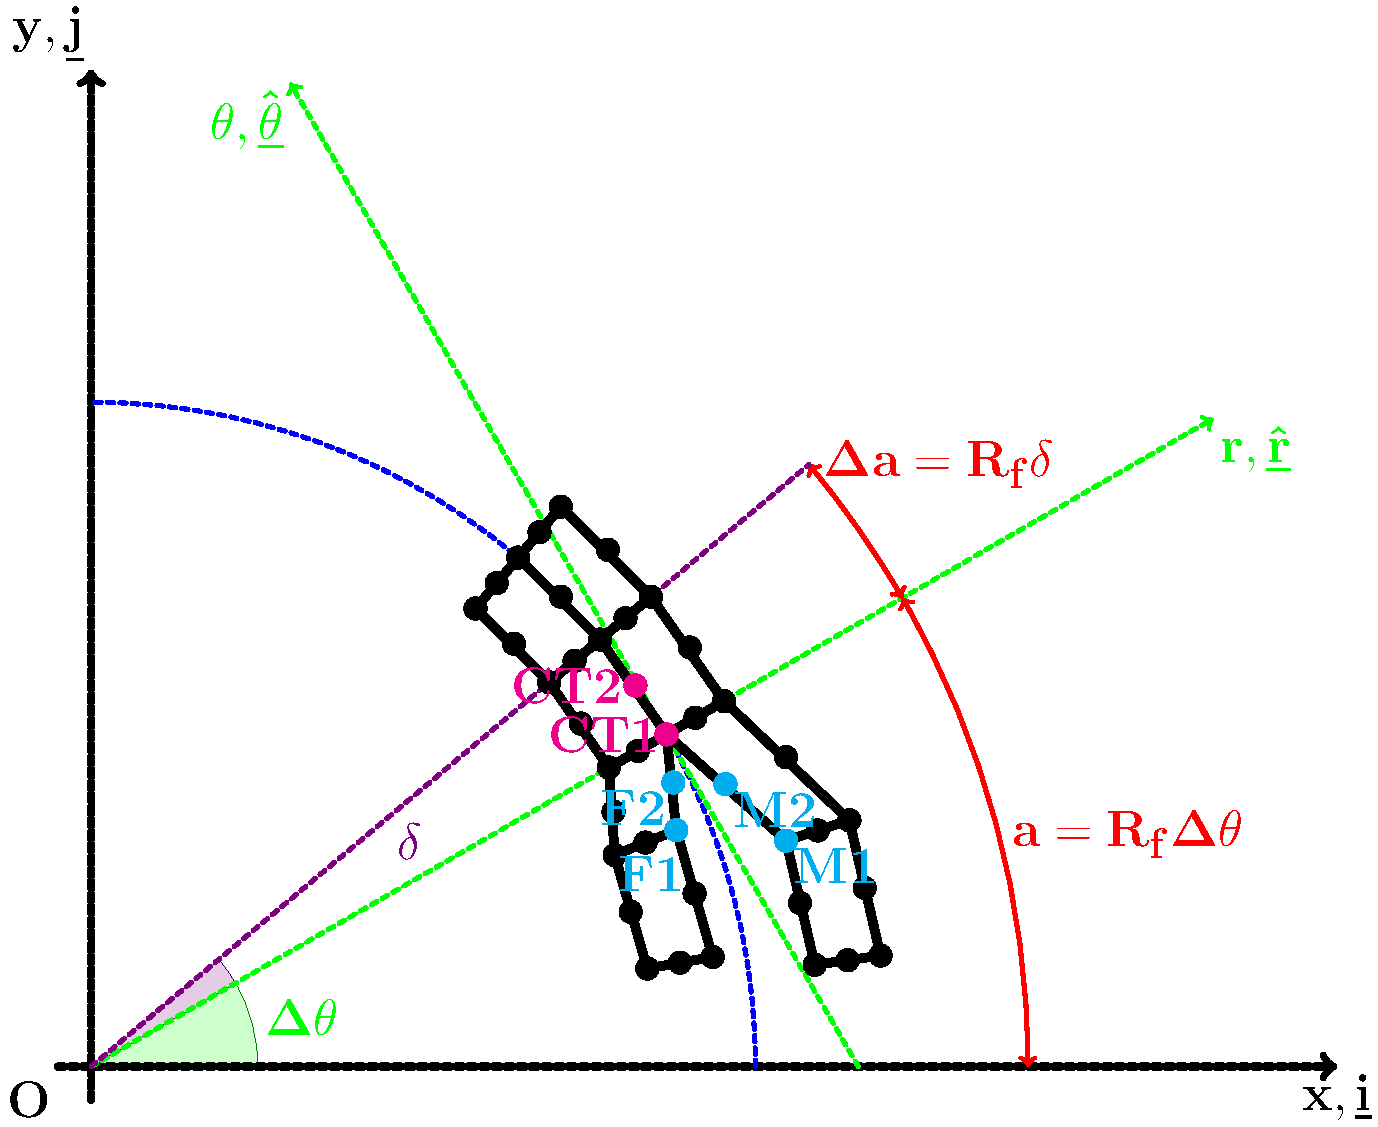
\includegraphics[width=\textwidth]{VCCT-quadratic.pdf}
\caption{Schematic representation of the discretized crack tip geometry for $2^{nd}$ order quadrilateral elements.}
\end{figure}

\begin{equation}
\underline{\underline{R}}=\begin{bmatrix}
\cos\left(\Delta\theta\right) & \sin\left(\Delta\theta\right) \\
-\sin\left(\Delta\theta\right) & \cos\left(\Delta\theta\right)
\end{bmatrix}\qquad\underline{\underline{R}}^{-1}=\underline{\underline{R}}^{T}=\begin{bmatrix}
\cos\left(\Delta\theta\right) & -\sin\left(\Delta\theta\right) \\
\sin\left(\Delta\theta\right) & \cos\left(\Delta\theta\right)
\end{bmatrix}
\end{equation}

\begin{equation}
\begin{bmatrix}
r \\
\theta
\end{bmatrix}=\underline{\underline{R}}\begin{bmatrix}
x \\
y
\end{bmatrix}\qquad\begin{bmatrix}
x \\
y
\end{bmatrix}=\underline{\underline{R}}^{-1}\begin{bmatrix}
r \\
\theta
\end{bmatrix}
\end{equation}

\subsection{Calculation of displacements and reaction forces}

\begin{equation}
\begin{split}
u_{x,1}=u_{x,M1}-u_{x,F1}&\qquad u_{y,1}=u_{y,M1}-u_{y,F1}\\
u_{x,2}=u_{x,M2}-u_{x,F2}&\qquad u_{y,2}=u_{y,M2}-u_{y,F2}
\end{split}
\end{equation}

\begin{equation}
\begin{split}
u_{r,1}=\cos\left(\Delta\theta\right) u_{x,1}+\sin\left(\Delta\theta\right) u_{y,1}&\qquad u_{\theta,1}=-\sin\left(\Delta\theta\right) u_{x,1}+\cos\left(\Delta\theta\right) u_{y,1}\\
u_{r,2}=\cos\left(\Delta\theta\right) u_{x,2}+\sin\left(\Delta\theta\right) u_{y,2}&\qquad u_{\theta,2}=-\sin\left(\Delta\theta\right) u_{x,2}+\cos\left(\Delta\theta\right) u_{y,2}
\end{split}
\end{equation}

\begin{equation}
\begin{split}
F_{r,1}=\cos\left(\Delta\theta\right) F_{x,1}+\sin\left(\Delta\theta\right) F_{y,1}&\qquad F_{\theta,1}=-\sin\left(\Delta\theta\right) F_{x,1}+\cos\left(\Delta\theta\right) F_{y,1}\\
F_{r,2}=\cos\left(\Delta\theta\right) F_{x,2}+\sin\left(\Delta\theta\right) F_{y,2}&\qquad F_{\theta,2}=-\sin\left(\Delta\theta\right) F_{x,2}+\cos\left(\Delta\theta\right) F_{y,2}\\
\end{split}
\end{equation}

\subsection{Calculation of energy release rates}

\begin{equation}
\begin{split}
G_{I,r\theta} = &\frac{1}{2R_{f}\delta}\left(F_{r,1}u_{r,1}+F_{r,2}u_{r,2}\right)=\\
= &\frac{1}{2R_{f}\delta}\left(\cos\left(\Delta\theta\right) F_{x,1}+\sin\left(\Delta\theta\right)F_{y,1}\right)\left(\cos\left(\Delta\theta\right) u_{x,1}+\sin\left(\Delta\theta\right) u_{y,1}\right)+\\
&+\frac{1}{2R_{f}\delta}\left(\cos\left(\Delta\theta\right) F_{x,2}+\sin\left(\Delta\theta\right)F_{y,2}\right)\left(\cos\left(\Delta\theta\right) u_{x,2}+\sin\left(\Delta\theta\right) u_{y,2}\right)+\\
= &\frac{1}{2R_{f}\delta}\left(\cos^{2}\left(\Delta\theta\right) F_{x,1}u_{x,1}+\left(F_{x,1}u_{y,1}+F_{y,1}u_{x,1}\right)\cos\left(\Delta\theta\right)\sin\left(\Delta\theta\right)+\sin^{2}\left(\Delta\theta\right)F_{y,1}u_{y,1}\right)+\\
&+\frac{1}{2R_{f}\delta}\left(\cos^{2}\left(\Delta\theta\right) F_{x,2}u_{x,2}+\left(F_{x,2}u_{y,2}+F_{y,2}u_{x,2}\right)\cos\left(\Delta\theta\right)\sin\left(\Delta\theta\right)+\sin^{2}\left(\Delta\theta\right)F_{y,2}u_{y,2}\right)
\end{split}
\end{equation}

\begin{equation}
\begin{split}
G_{II,r\theta} = &\frac{1}{2R_{f}\delta}\left(F_{\theta,1}u_{\theta,1}+F_{\theta,2}u_{\theta,2}\right)=\\
= &\frac{1}{2R_{f}\delta}\left(-\sin\left(\Delta\theta\right) F_{x,1}+\cos\left(\Delta\theta\right)F_{y,1}\right)\left(-\sin\left(\Delta\theta\right) u_{x,1}+\cos\left(\Delta\theta\right) u_{y,1}\right)+\\
&+\frac{1}{2R_{f}\delta}\left(-\sin\left(\Delta\theta\right) F_{x,2}+\cos\left(\Delta\theta\right)F_{y,2}\right)\left(-\sin\left(\Delta\theta\right) u_{x,2}+\cos\left(\Delta\theta\right) u_{y,2}\right)=\\
= &\frac{1}{2R_{f}\delta}\left(\sin^{2}\left(\Delta\theta\right) F_{x,1}u_{x,1}-\left(F_{x,1}u_{y,1}+F_{y,1}u_{x,1}\right)\cos\left(\Delta\theta\right)\sin\left(\Delta\theta\right)+\cos^{2}\left(\Delta\theta\right)F_{y,1}u_{y,1}\right)+\\
 &+\frac{1}{2R_{f}\delta}\left(\sin^{2}\left(\Delta\theta\right) F_{x,2}u_{x,2}-\left(F_{x,2}u_{y,2}+F_{y,2}u_{x,2}\right)\cos\left(\Delta\theta\right)\sin\left(\Delta\theta\right)+\cos^{2}\left(\Delta\theta\right)F_{y,2}u_{y,2}\right)\\
\end{split}
\end{equation}

\begin{equation}
\begin{split}
G_{TOT,r\theta} = &G_{I,r\theta} + G_{II,r\theta}=\\
=&\frac{1}{2R_{f}\delta}\left(\cos^{2}\left(\Delta\theta\right) F_{x,1}u_{x,1}+\left(F_{x,1}u_{y,1}+F_{y,1}u_{x,1}\right)\cos\left(\Delta\theta\right)\sin\left(\Delta\theta\right)+\sin^{2}\left(\Delta\theta\right)F_{y,1}u_{y,1}\right)+\\
&+\frac{1}{2R_{f}\delta}\left(\cos^{2}\left(\Delta\theta\right) F_{x,2}u_{x,2}+\left(F_{x,2}u_{y,2}+F_{y,2}u_{x,2}\right)\cos\left(\Delta\theta\right)\sin\left(\Delta\theta\right)+\sin^{2}\left(\Delta\theta\right)F_{y,2}u_{y,2}\right)+\\
&+\frac{1}{2R_{f}\delta}\left(\sin^{2}\left(\Delta\theta\right) F_{x,1}u_{x,1}-\left(F_{x,1}u_{y,1}+F_{y,1}u_{x,1}\right)\cos\left(\Delta\theta\right)\sin\left(\Delta\theta\right)+\cos^{2}\left(\Delta\theta\right)F_{y,1}u_{y,1}\right)+\\
 &+\frac{1}{2R_{f}\delta}\left(\sin^{2}\left(\Delta\theta\right) F_{x,2}u_{x,2}-\left(F_{x,2}u_{y,2}+F_{y,2}u_{x,2}\right)\cos\left(\Delta\theta\right)\sin\left(\Delta\theta\right)+\cos^{2}\left(\Delta\theta\right)F_{y,2}u_{y,2}\right)=\\
= &\frac{1}{2R_{f}\delta}\cos^{2}\left(\Delta\theta\right) \left(F_{x,1}u_{x,1}+F_{x,2}u_{x,2}+F_{y,1}u_{y,1}+F_{y,2}u_{y,2}\right)+\\
&+\frac{1}{2R_{f}\delta}\left(\left(F_{x,1}u_{y,1}+F_{x,1}u_{y,1}\right)+\left(F_{y,2}u_{x,2}+F_{y,2}u_{x,2}\right)\right)\cos\left(\Delta\theta\right)\sin\left(\Delta\theta\right)+\\
&+\frac{1}{2R_{f}\delta}\sin^{2}\left(\Delta\theta\right)\left(F_{x,1}u_{x,1}+F_{x,2}u_{x,2}+F_{y,1}u_{y,1}+F_{y,2}u_{y,2}\right)+\\
&-\frac{1}{2R_{f}\delta}\left(\left(F_{x,1}u_{y,1}+F_{x,1}u_{y,1}\right)+\left(F_{y,2}u_{x,2}+F_{y,2}u_{x,2}\right)\right)\cos\left(\Delta\theta\right)\sin\left(\Delta\theta\right)=\\
=&\frac{1}{2R_{f}\delta}\left(\cancelto{1}{\left(\cos^{2}\left(\Delta\theta\right)+\sin^{2}\left(\Delta\theta\right)\right)}\left(F_{x,1}u_{x,1}+F_{x,2}u_{x,2}\right)\right)+\\
&+\frac{1}{2R_{f}\delta}\cancelto{0}{\left(\left(F_{x,1}u_{y,1}+F_{x,1}u_{y,1}\right)-\left(F_{x,1}u_{y,1}+F_{x,1}u_{y,1}\right)\right)}\cos\left(\Delta\theta\right)\sin\left(\Delta\theta\right)+\\
&+\frac{1}{2R_{f}\delta}\cancelto{0}{\left(\left(F_{y,2}u_{x,2}+F_{y,2}u_{x,2}\right)-\left(F_{y,2}u_{x,2}+F_{y,2}u_{x,2}\right)\right)}\cos\left(\Delta\theta\right)\sin\left(\Delta\theta\right)+\\
&+\frac{1}{2R_{f}\delta}\left(\cancelto{1}{\left(\cos^{2}\left(\Delta\theta\right)+\sin^{2}\left(\Delta\theta\right)\right)}\left(F_{y,1}u_{y,1}+F_{y,2}u_{y,2}\right)\right)=\\
=&\frac{1}{2}\frac{F_{x,1}u_{x,1}+F_{x,2}u_{x,2}}{R_{f}\delta}+\frac{1}{2}\frac{F_{y,1}u_{y,1}+F_{y,2}u_{y,2}}{R_{f}\delta}=\\
=&\widetilde{G}_{I,xy} + \widetilde{G}_{II,xy}=\widetilde{G}_{TOT,xy}
\end{split}
\end{equation}

\begin{equation}
\begin{split}
G_{I,r\theta} = &\cos^{2}\left(\Delta\theta\right)\frac{F_{x,1}u_{x,1}+F_{x,2}u_{x,2}}{2R_{f}\delta}+\\
&+\frac{F_{x,1}u_{y,1}+F_{y,1}u_{x,1}+F_{x,2}u_{y,2}+F_{y,2}u_{x,2}}{2R_{f}\delta}\cos\left(\Delta\theta\right)\sin\left(\Delta\theta\right)+\\
&+\sin^{2}\left(\Delta\theta\right)\frac{F_{y,1}u_{y,1}+F_{y,2}u_{y,2}}{2R_{f}\delta}=\\
=&\cos^{2}\left(\Delta\theta\right)\widetilde{G}_{I,xy}+\sin^{2}\left(\Delta\theta\right)\widetilde{G}_{II,xy}+\\
&+\frac{F_{x,1}u_{y,1}+F_{y,1}u_{x,1}+F_{x,2}u_{y,2}+F_{y,2}u_{x,2}}{2R_{f}\delta}\cos\left(\Delta\theta\right)\sin\left(\Delta\theta\right)
\end{split}
\end{equation}

\begin{equation}
\begin{split}
G_{II,r\theta} = &\sin^{2}\left(\Delta\theta\right)\frac{F_{x,1}u_{x,1}+F_{x,2}u_{x,2}}{2R_{f}\delta}+\\
&-\frac{F_{x,1}u_{y,1}+F_{y,1}u_{x,1}+F_{x,2}u_{y,2}+F_{y,2}u_{x,2}}{2R_{f}\delta}\cos\left(\Delta\theta\right)\sin\left(\Delta\theta\right)+\\
&+\cos^{2}\left(\Delta\theta\right)\frac{F_{y,1}u_{y,1}+F_{y,2}u_{y,2}}{2R_{f}\delta}=\\
=&\sin^{2}\left(\Delta\theta\right)\widetilde{G}_{I,xy}+\cos^{2}\left(\Delta\theta\right)\widetilde{G}_{II,xy}+\\
&-\frac{F_{x,1}u_{y,1}+F_{y,1}u_{x,1}+F_{x,2}u_{y,2}+F_{y,2}u_{x,2}}{2R_{f}\delta}\cos\left(\Delta\theta\right)\sin\left(\Delta\theta\right)
\end{split}
\end{equation}

\subsection{Sensitivity analysis of the FEM solution}

\begin{equation}
\begin{split}
F_{x,1}\sim k_{x,1}u_{x,1}&\qquad F_{y,1}\sim k_{y,1}u_{y,1}\\
F_{x,2}\sim k_{x,2}u_{x,2}&\qquad F_{y,2}\sim k_{y,2}u_{y,2}\\
\end{split}
\end{equation}

\begin{equation}
\begin{split}
G_{I,r\theta} \sim &\frac{1}{2R_{f}\delta}\cos^{2}\left(\Delta\theta\right)\left(k_{x,1}u^{2}_{x,1}+k_{x,2}u^{2}_{x,2}\right)+\\
&+\frac{1}{2R_{f}\delta}\cos\left(\Delta\theta\right)\sin\left(\Delta\theta\right)\left(k_{x,1}u_{x,1}u_{y,1}+k_{y,1}u_{y,1}u_{x,1}+k_{x,2}u_{x,2}u_{y,2}+k_{y,2}u_{y,2}u_{x,2}\right)+\\
&+\frac{1}{2R_{f}\delta}\sin^{2}\left(\Delta\theta\right)\left(k_{y,1}u^{2}_{y,1}+k_{y,2}u^{2}_{y,2}\right)
\end{split}
\end{equation}

\begin{equation}
\begin{split}
G_{II,r\theta} \sim &\frac{1}{2R_{f}\delta}\sin^{2}\left(\Delta\theta\right)\left(k_{x,1}u^{2}_{x,1}+k_{x,2}u^{2}_{x,2}\right)+\\
&-\frac{1}{2R_{f}\delta}\cos\left(\Delta\theta\right)\sin\left(\Delta\theta\right)\left(k_{x,1}u_{x,1}u_{y,1}+k_{y,1}u_{y,1}u_{x,1}+k_{x,2}u_{x,2}u_{y,2}+k_{y,2}u_{y,2}u_{x,2}\right)+\\
&+\frac{1}{2R_{f}\delta}\cos^{2}\left(\Delta\theta\right)\left(k_{y,1}u^{2}_{y,1}+k_{y,2}u^{2}_{y,2}\right)
\end{split}
\end{equation}

\begin{equation}
\begin{split}
G_{TOT,r\theta} \sim &\frac{1}{2R_{f}\delta}\left(\left(k_{x,1}u^{2}_{x,1}\left(\Delta\theta\right)+k_{x,2}u^{2}_{x,2}\left(\Delta\theta\right)\right)+\left(k_{y,1}u^{2}_{y,1}\left(\Delta\theta\right)+k_{y,2}u^{2}_{y,2}\left(\Delta\theta\right)\right)\right)
\end{split}
\end{equation}

\begin{equation}
\begin{split}
\frac{\partial G_{I,r\theta}}{\partial\Delta\theta} \sim&\frac{1}{R_{f}\delta}\cos^{2}\left(\Delta\theta\right)\left( k_{x,1}u_{x,1}\left(\Delta\theta\right)\frac{\partial u_{x,1}\left(\Delta\theta\right)}{\partial\Delta\theta}+k_{x,2}u_{x,2}\left(\Delta\theta\right)\frac{\partial u_{x,2}\left(\Delta\theta\right)}{\partial\Delta\theta}\right)+\\
&+\frac{1}{2R_{f}\delta}\left(k_{x,1}+k_{y,1}\right)\left(\frac{\partial u_{x,1}\left(\Delta\theta\right)}{\partial\Delta\theta}u_{y,1}\left(\Delta\theta\right)+u_{x,1}\left(\Delta\theta\right)\frac{\partial u_{y,1}\left(\Delta\theta\right)}{\partial\Delta\theta}\right)\cos\left(\Delta\theta\right)\sin\left(\Delta\theta\right)+\\
&+\frac{1}{2R_{f}\delta}\left(k_{x,2}+k_{y,2}\right)\left(\frac{\partial u_{x,2}\left(\Delta\theta\right)}{\partial\Delta\theta}u_{y,2}\left(\Delta\theta\right)+u_{x,2}\left(\Delta\theta\right)\frac{\partial u_{y,2}\left(\Delta\theta\right)}{\partial\Delta\theta}\right)\cos\left(\Delta\theta\right)\sin\left(\Delta\theta\right)+\\
&+\frac{1}{R_{f}\delta}\sin^{2}\left(\Delta\theta\right)\left(k_{y,1}u_{y,1}\left(\Delta\theta\right)\frac{\partial u_{y,1}\left(\Delta\theta\right)}{\partial\Delta\theta}+k_{y,2}u_{y,2}\left(\Delta\theta\right)\frac{\partial u_{y,2}\left(\Delta\theta\right)}{\partial\Delta\theta}\right)+\\
&+\frac{1}{2R_{f}\delta}\left(\left(k_{y,1}u^{2}_{y,1}+k_{y,2}u^{2}_{y,2}\right)-\left(k_{x,1}u^{2}_{x,1}+k_{x,2}u^{2}_{x,2}\right)\right)\sin\left(2\Delta\theta\right)+\\
&+\frac{1}{2R_{f}\delta}\left(\left(k_{x,1}+k_{y,1}\right)u_{x,1}u_{y,1}+\left(k_{x,2}+k_{y,2}\right)u_{x,2}u_{y,2}\right)\cos\left(2\Delta\theta\right)\\
\end{split}
\end{equation}

\begin{equation}
\begin{split}
\frac{\partial G_{II,r\theta}}{\partial\Delta\theta} \sim&\frac{1}{R_{f}\delta}\sin^{2}\left(\Delta\theta\right)\left( k_{x,1}u_{x,1}\left(\Delta\theta\right)\frac{\partial u_{x,1}\left(\Delta\theta\right)}{\partial\Delta\theta}+k_{x,2}u_{x,2}\left(\Delta\theta\right)\frac{\partial u_{x,2}\left(\Delta\theta\right)}{\partial\Delta\theta}\right)+\\
&-\frac{1}{2R_{f}\delta}\left(k_{x,1}+k_{y,1}\right)\left(\frac{\partial u_{x,1}\left(\Delta\theta\right)}{\partial\Delta\theta}u_{y,1}\left(\Delta\theta\right)+u_{x,1}\left(\Delta\theta\right)\frac{\partial u_{y,1}\left(\Delta\theta\right)}{\partial\Delta\theta}\right)\cos\left(\Delta\theta\right)\sin\left(\Delta\theta\right)+\\
&-\frac{1}{2R_{f}\delta}\left(k_{x,2}+k_{y,2}\right)\left(\frac{\partial u_{x,2}\left(\Delta\theta\right)}{\partial\Delta\theta}u_{y,2}\left(\Delta\theta\right)+u_{x,2}\left(\Delta\theta\right)\frac{\partial u_{y,2}\left(\Delta\theta\right)}{\partial\Delta\theta}\right)\cos\left(\Delta\theta\right)\sin\left(\Delta\theta\right)+\\
&+\frac{1}{R_{f}\delta}\cos^{2}\left(\Delta\theta\right)\left(k_{y,1}u_{y,1}\left(\Delta\theta\right)\frac{\partial u_{y,1}\left(\Delta\theta\right)}{\partial\Delta\theta}+k_{y,2}u_{y,2}\left(\Delta\theta\right)\frac{\partial u_{y,2}\left(\Delta\theta\right)}{\partial\Delta\theta}\right)+\\
&+\frac{1}{2R_{f}\delta}\left(\left(k_{x,1}u^{2}_{x,1}+k_{x,2}u^{2}_{x,2}\right)-\left(k_{y,1}u^{2}_{y,1}+k_{y,2}u^{2}_{y,2}\right)\right)\sin\left(2\Delta\theta\right)+\\
&-\frac{1}{2R_{f}\delta}\left(\left(k_{x,1}+k_{y,1}\right)u_{x,1}u_{y,1}+\left(k_{x,2}+k_{y,2}\right)u_{x,2}u_{y,2}\right)\cos\left(2\Delta\theta\right)\\
\end{split}
\end{equation}

\begin{equation}
\begin{split}
G_{TOT,r\theta} \sim &\frac{1}{R_{f}\delta}\left(\left( k_{x,1}u_{x,1}\frac{\partial u_{x,1}}{\partial\Delta\theta}+k_{x,2}u_{x,2}\frac{\partial u_{x,2}}{\partial\Delta\theta}\right)+\left(k_{y,1}u_{y,1}\frac{\partial u_{y,1}}{\partial\Delta\theta}+k_{y,2}u_{y,2}\frac{\partial u_{y,2}}{\partial\Delta\theta}\right)\right)
\end{split}
\end{equation}

\clearpage

\section{A vectorial formulation of the VCCT}

\subsection{Vectorial formulation}

\begin{equation}
\underline{\underline{R}}_{\Delta\theta}=\begin{bmatrix}
\cos\left(\Delta\theta\right) & \sin\left(\Delta\theta\right) \\
-\sin\left(\Delta\theta\right) & \cos\left(\Delta\theta\right)
\end{bmatrix}\qquad\underline{\underline{R}}_{\Delta\theta}^{-1}=\underline{\underline{R}}^{T}=\begin{bmatrix}
\cos\left(\Delta\theta\right) & -\sin\left(\Delta\theta\right) \\
\sin\left(\Delta\theta\right) & \cos\left(\Delta\theta\right)
\end{bmatrix}
\end{equation}

\begin{equation}
\underline{\underline{R}}_{\delta}=\begin{bmatrix}
\cos\left(\delta\right) & \sin\left(\delta\right) \\
-\sin\left(\delta\right) & \cos\left(\delta\right)
\end{bmatrix}\qquad\underline{\underline{R}}_{\delta}^{-1}=\underline{\underline{R}}_{\delta}^{T}=\begin{bmatrix}
\cos\left(\delta\right) & -\sin\left(\delta\right) \\
\sin\left(\delta\right) & \cos\left(\delta\right)
\end{bmatrix}
\end{equation}

\begin{equation}
\frac{\partial \underline{\underline{R}}_{\Delta\theta}}{\partial \Delta\theta}=\underline{\underline{D}}\cdot\underline{\underline{R}}_{\Delta\theta}
\end{equation}

\begin{equation}
\frac{\partial \underline{\underline{R}}_{\delta}}{\partial \delta}=\underline{\underline{D}}\cdot\underline{\underline{R}}_{\delta}
\end{equation}

\begin{equation}
\underline{\underline{D}}=\begin{bmatrix}
0 & 1\\
-1& 0
\end{bmatrix}
\end{equation}

\begin{equation}
\underline{F}_{xy}=\begin{bmatrix}
F_{x} \\
F_{y}
\end{bmatrix}\qquad\underline{F}_{r\theta}=\begin{bmatrix}
F_{r} \\
F_{\theta}
\end{bmatrix}
\end{equation}

\begin{equation}
\underline{u}_{xy}=\begin{bmatrix}
u_{x} \\
u_{y}
\end{bmatrix}\qquad\underline{u}_{r\theta}=\begin{bmatrix}
u_{r} \\
u_{\theta}
\end{bmatrix}
\end{equation}

\begin{equation}
\underline{G}=\begin{bmatrix}
G_{I} \\
G_{II}
\end{bmatrix}
\end{equation}

\begin{equation}
\underline{F}_{r\theta}=\underline{\underline{R}}_{\Delta\theta}\underline{F}_{xy}\qquad\underline{u}_{r\theta}=\underline{\underline{R}}_{\delta}\underline{\underline{R}}_{\Delta\theta}\underline{u}_{xy}
\end{equation}

\begin{equation}
\underline{F}_{xy}=\underline{\underline{K}}_{xy}\underline{u}_{xy}+\underline{\widetilde{F}}_{xy}=\underline{\underline{K}}_{xy}\underline{u}_{xy}+\underline{\underline{\widetilde{K}}}_{N}\underline{u}_{N}
\end{equation}

\begin{equation}
\begin{split}
G_{TOT} &= \frac{1}{2R_{f}\delta}\underline{u}_{r\theta}^{T}\underline{F}_{r\theta}=\\
&=\frac{1}{2R_{f}\delta}Tr\left(\underline{F}_{r\theta}\underline{u}_{r\theta}^{T}\right)=\frac{1}{2R_{f}\delta}Tr\left(\begin{bmatrix}
F_{r}u_{r}&F_{r}u_{\theta}\\
F_{\theta}u_{r}&F_{\theta}u_{\theta}\\
\end{bmatrix}\right)=\\
&=\frac{1}{2R_{f}\delta}Tr\left(\underline{\underline{R}}_{\Delta\theta}\underline{F}_{xy}\underline{u}_{xy}^{T}\underline{\underline{R}}_{\Delta\theta}^{T}\underline{\underline{R}}_{\delta}^{T}\right)
\end{split}
\end{equation}

\begin{equation}
\begin{split}
G_{TOT} &= \frac{1}{2R_{f}\delta}Tr\left(\underline{\underline{R}}_{\Delta\theta}\left(\underline{\underline{K}}_{xy}\underline{u}_{xy}+\underline{\widetilde{F}}_{xy}\right)\underline{u}_{xy}^{T}\underline{\underline{R}}_{\Delta\theta}^{T}\underline{\underline{R}}_{\delta}^{T}\right)=\\
&=\frac{1}{2R_{f}\delta}Tr\left(\underline{\underline{R}}_{\Delta\theta}\underline{\underline{K}}_{xy}\underline{u}_{xy}\underline{u}_{xy}^{T}\underline{\underline{R}}_{\Delta\theta}^{T}\underline{\underline{R}}_{\delta}^{T}\right)+\frac{1}{2R_{f}\delta}Tr\left(\underline{\underline{R}}_{\Delta\theta}\underline{\widetilde{F}}_{xy}\underline{u}_{xy}^{T}\underline{\underline{R}}_{\Delta\theta}^{T}\underline{\underline{R}}_{\delta}^{T}\right)\\
\end{split}
\end{equation}

\begin{equation}
\underline{G}=\begin{bmatrix}
G_{I} \\
G_{II}
\end{bmatrix}=\frac{1}{2R_{f}\delta}Diag\left(\underline{\underline{R}}_{\Delta\theta}\underline{F}_{xy}\underline{u}_{xy}^{T}\underline{\underline{R}}_{\Delta\theta}^{T}\underline{\underline{R}}_{\delta}^{T}\right)
\end{equation}

\begin{equation}
\begin{split}
\underline{G}=\begin{bmatrix}
G_{I} \\
G_{II}
\end{bmatrix}=&\frac{1}{2R_{f}\delta}Diag\left(\underline{\underline{R}}_{\Delta\theta}\underline{\underline{K}}_{xy}\underline{u}_{xy}\underline{u}_{xy}^{T}\underline{\underline{R}}_{\Delta\theta}^{T}\underline{\underline{R}}_{\delta}^{T}\right)+\frac{1}{2R_{f}\delta}Diag\left(\underline{\underline{R}}_{\Delta\theta}\underline{\widetilde{F}}_{xy}\underline{u}_{xy}^{T}\underline{\underline{R}}_{\Delta\theta}^{T}\underline{\underline{R}}_{\delta}^{T}\right)=\\
=&\frac{1}{2R_{f}\delta}Diag\left(\underline{\underline{R}}_{\Delta\theta}\underline{\underline{K}}_{xy}\underline{u}_{xy}\underline{u}_{xy}^{T}\underline{\underline{R}}_{\Delta\theta}^{T}\underline{\underline{R}}_{\delta}^{T}\right)+\frac{1}{2R_{f}\delta}Diag\left(\underline{\underline{R}}_{\Delta\theta}\underline{\underline{\widetilde{K}}}_{N}\underline{u}_{N}\underline{u}_{xy}^{T}\underline{\underline{R}}_{\Delta\theta}^{T}\underline{\underline{R}}_{\delta}^{T}\right)
\end{split}
\end{equation}

\subsection{Sensitivity analysis}

\begin{equation}
\begin{split}
\frac{\partial \underline{G}}{\partial \delta}=&-\frac{1}{2R_{f}\delta^{2}}Diag\left(\underline{\underline{R}}_{\Delta\theta}\underline{\underline{K}}_{xy}\underline{u}_{xy}\underline{u}_{xy}^{T}\underline{\underline{R}}_{\Delta\theta}^{T}\underline{\underline{R}}_{\delta}^{T}\right)-\frac{1}{2R_{f}\delta^{2}}Diag\left(\underline{\underline{R}}_{\Delta\theta}\underline{\underline{\widetilde{K}}}_{N}\underline{u}_{N}\underline{u}_{xy}^{T}\underline{\underline{R}}_{\Delta\theta}^{T}\underline{\underline{R}}_{\delta}^{T}\right)+\\
+&\frac{1}{2R_{f}\delta}Diag\left(\underline{\underline{R}}_{\Delta\theta}\underline{\underline{K}}_{xy}\underline{u}_{xy}\underline{u}_{xy}^{T}\underline{\underline{R}}_{\Delta\theta}^{T}\underline{\underline{R}}_{\delta}^{T}\underline{\underline{D}}^{T}\right)+\frac{1}{2R_{f}\delta}Diag\left(\underline{\underline{R}}_{\Delta\theta}\underline{\underline{\widetilde{K}}}_{N}\underline{u}_{N}\underline{u}_{xy}^{T}\underline{\underline{R}}_{\Delta\theta}^{T}\underline{\underline{R}}_{\delta}^{T}\underline{\underline{D}}^{T}\right)+\\
+&\frac{1}{2R_{f}\delta}Diag\left(\underline{\underline{R}}_{\Delta\theta}\underline{\underline{K}}_{xy}\frac{\partial \underline{u}_{xy}}{\partial \delta}\underline{u}_{xy}^{T}\underline{\underline{R}}_{\Delta\theta}^{T}\underline{\underline{R}}_{\delta}^{T}\right)+\frac{1}{2R_{f}\delta}Diag\left(\underline{\underline{R}}_{\Delta\theta}\underline{\underline{\widetilde{K}}}_{N}\frac{\partial \underline{u}_{N}}{\partial \delta}\underline{u}_{xy}^{T}\underline{\underline{R}}_{\Delta\theta}^{T}\underline{\underline{R}}_{\delta}^{T}\right)+\\
+&\frac{1}{2R_{f}\delta}Diag\left(\underline{\underline{R}}_{\Delta\theta}\underline{\underline{K}}_{xy}\underline{u}_{xy}\frac{\partial \underline{u}_{xy}^{T}}{\partial \delta}\underline{\underline{R}}_{\Delta\theta}^{T}\underline{\underline{R}}_{\delta}^{T}\right)+\frac{1}{2R_{f}\delta}Diag\left(\underline{\underline{R}}_{\Delta\theta}\underline{\underline{\widetilde{K}}}_{N}\underline{u}_{N}\frac{\partial \underline{u}_{xy}^{T}}{\partial \delta}\underline{\underline{R}}_{\Delta\theta}^{T}\underline{\underline{R}}_{\delta}^{T}\right)=\\
=&\frac{1}{\delta}\underline{G}+Diag\left(\frac{1}{2R_{f}\delta}\underline{\underline{R}}_{\Delta\theta}\left(\underline{\underline{K}}_{xy}\underline{u}_{xy}+\underline{\underline{\widetilde{K}}}_{N}\underline{u}_{N}\right)\underline{u}_{xy}^{T}\underline{\underline{R}}_{\Delta\theta}^{T}\underline{\underline{R}}_{\delta}^{T}\underline{\underline{D}}^{T}\right)+\\
+&\frac{1}{R_{f}\delta}Diag\left(\underline{\underline{R}}_{\Delta\theta}\underline{\underline{K}}_{xy}\frac{\partial \underline{u}_{xy}}{\partial \delta}\underline{u}_{xy}^{T}\underline{\underline{R}}_{\Delta\theta}^{T}\underline{\underline{R}}_{\delta}^{T}\right)+\frac{1}{2R_{f}\delta}Diag\left(\underline{\underline{R}}_{\Delta\theta}\underline{\underline{\widetilde{K}}}_{N}\frac{\partial \underline{u}_{N}}{\partial \delta}\underline{u}_{xy}^{T}\underline{\underline{R}}_{\Delta\theta}^{T}\underline{\underline{R}}_{\delta}^{T}\right)+\\
+&\frac{1}{2R_{f}\delta}Diag\left(\underline{\underline{R}}_{\Delta\theta}\underline{\underline{\widetilde{K}}}_{N}\underline{u}_{N}\frac{\partial \underline{u}_{xy}^{T}}{\partial \delta}\underline{\underline{R}}_{\Delta\theta}^{T}\underline{\underline{R}}_{\delta}^{T}\right)
\end{split}
\end{equation}

Following Comninou

\begin{equation}
u\left(\delta\right)\sim \sqrt{\delta}\left(\sin,\cos\right)\left(\epsilon\log{\delta}\right)\qquad\epsilon=\frac{1}{2\pi}\log{\left(\frac{1-\beta}{1+\beta}\right)}
\end{equation}

\begin{equation}
\underline{u}_{xy},\underline{u}_{N}\sim u\left(\delta\right)\sim\sqrt{\delta}\left(\sin,\cos\right)\left(\epsilon\log{\delta}\right)\xrightarrow{\delta\rightarrow 0}0
\end{equation}

\begin{equation}
\underline{u}_{xy}\underline{u}_{xy}^{T},\underline{u}_{N}\underline{u}_{xy}^{T}\sim u^{2}\left(\delta\right)\sim\delta\left(\sin^{2},\cos^{2},\sin\cdot\cos\right)\left(\epsilon\log{\delta}\right)\xrightarrow{\delta\rightarrow 0}0
\end{equation}

\begin{equation}
\frac{\partial \underline{u}_{xy}}{\partial \delta}\underline{u}_{xy}^{T},\frac{\partial \underline{u}_{N}}{\partial \delta}\underline{u}_{xy}^{T}\sim -\frac{1}{2}\left(\sin^{2},\cos^{2},\sin\cdot\cos\right)\left(\epsilon\log{\delta}\right)+\left(-\sin^{2},\cos^{2},\pm\sin\cdot\cos\right)\left(\epsilon\log{\delta}\right)\xrightarrow{\delta\rightarrow 0}finite
\end{equation}

\begin{equation}
\underline{G}\sim\frac{1}{\delta}\underline{u}_{xy}\underline{u}_{xy}^{T}\sim \frac{1}{\delta}u^{2}\left(\delta\right)\sim\left(\sin^{2},\cos^{2},\sin\cdot\cos\right)\left(\epsilon\log{\delta}\right)\xrightarrow{\delta\rightarrow 0}finite
\end{equation}

\begin{equation}
\lim_{\delta\rightarrow 0}\frac{\partial \underline{G}}{\partial \delta}\sim\frac{1}{\delta}\left(\cancelto{0}{\underline{F}\left(\delta\right)}+\underline{C}\right)
\end{equation}

\begin{equation}
\lim_{\delta\rightarrow 0}\frac{\partial \underline{G}}{\partial \delta}\sim\frac{1}{\delta}\quad\xrightarrow{\int d\delta}\quad\lim_{\delta\rightarrow 0}G\sim A\log(\delta)+B
\end{equation}

\begin{equation}
\begin{split}
\frac{\partial \underline{G}}{\partial \Delta\theta}=&\frac{1}{2R_{f}\delta}Diag\left(\underline{\underline{D}} \underline{\underline{R}}_{\Delta\theta}\underline{\underline{K}}_{xy}\underline{u}_{xy}\underline{u}_{xy}^{T}\underline{\underline{R}}_{\Delta\theta}^{T}\underline{\underline{R}}_{\delta}^{T}\right)+\frac{1}{2R_{f}\delta}Diag\left(\underline{\underline{D}}\underline{\underline{R}}_{\Delta\theta}\underline{\underline{\widetilde{K}}}_{N}\underline{u}_{N}\underline{u}_{xy}^{T}\underline{\underline{R}}_{\Delta\theta}^{T}\underline{\underline{R}}_{\delta}^{T}\right)+\\
+&\frac{1}{2R_{f}\delta}Diag\left(\underline{\underline{R}}_{\Delta\theta}\underline{\underline{K}}_{xy}\underline{u}_{xy}\underline{u}_{xy}^{T}\underline{\underline{R}}_{\Delta\theta}^{T}\underline{\underline{D}}^{T}\underline{\underline{R}}_{\delta}^{T}\right)+\frac{1}{2R_{f}\delta}Diag\left(\underline{\underline{R}}_{\Delta\theta}\underline{\underline{\widetilde{K}}}_{N}\underline{u}_{N}\underline{u}_{xy}^{T}\underline{\underline{R}}_{\Delta\theta}^{T}\underline{\underline{D}}^{T}\underline{\underline{R}}_{\delta}^{T}\right)+\\
+&\frac{1}{2R_{f}\delta}Diag\left(\underline{\underline{R}}_{\Delta\theta}\underline{\underline{K}}_{xy}\frac{\partial \underline{u}_{xy}}{\partial \Delta\theta}\underline{u}_{xy}^{T}\underline{\underline{R}}_{\Delta\theta}^{T}\underline{\underline{R}}_{\delta}^{T}\right)+\frac{1}{2R_{f}\delta}Diag\left(\underline{\underline{R}}_{\Delta\theta}\underline{\underline{\widetilde{K}}}_{N}\frac{\partial \underline{u}_{N}}{\partial \Delta\theta}\underline{u}_{xy}^{T}\underline{\underline{R}}_{\Delta\theta}^{T}\underline{\underline{R}}_{\delta}^{T}\right)+\\
+&\frac{1}{2R_{f}\delta}Diag\left(\underline{\underline{R}}_{\Delta\theta}\underline{\underline{K}}_{xy}\underline{u}_{xy}\frac{\partial \underline{u}_{xy}^{T}}{\partial \Delta\theta}\underline{\underline{R}}_{\Delta\theta}^{T}\underline{\underline{R}}_{\delta}^{T}\right)+\frac{1}{2R_{f}\delta}Diag\left(\underline{\underline{R}}_{\Delta\theta}\underline{\underline{\widetilde{K}}}_{N}\underline{u}_{N}\frac{\partial \underline{u}_{xy}^{T}}{\partial \Delta\theta}\underline{\underline{R}}_{\Delta\theta}^{T}\underline{\underline{R}}_{\delta}^{T}\right)\\
\end{split}
\end{equation}


\clearpage

%------------------------------------------------------------------------------------------%
%                             Interpolation
%------------------------------------------------------------------------------------------%

\section{Trigonometric interpolation}

By inspecting the results of the previous sections, an interpolation of the BEM results is performed manually by trial and error. The following procedure is followed:

\begin{enumerate}
\item a basis function is selected;
\item the frequency of the trigonometric basis function is calculated based on the position of the maximum value;
\item the amplitude is calculated based on the maximum value.
\end{enumerate}

\begin{figure}[!h]
\includegraphics[width=\textwidth]{Gsplot.pdf}
\caption{Interpolation of BEM results by manual trial and error.}
\end{figure}

The good agreement suggests that trigonometric functions are very good candidates for energy release rate data interpolation. The effect of different parameters can thus modeled as the functional variation of frequency (period) and amplitude of the trigonometric basis functions.

%\clearpage
%------------------------------------------------------------------------------------------%
%                             CONCLUSIONS AND PERSPECTIVES
%------------------------------------------------------------------------------------------%

%\section{Conclusions}


%------------------------------------------------------------------------------------------%
%                                   ACKNOWLEDGEMENTS
%------------------------------------------------------------------------------------------%
%\ack
%Luca Di Stasio gratefully acknowledges the support of the European School of Materials (EUSMAT) through the DocMASE Doctoral Programme and the European Commission through the Erasmus Mundus Programme.
%\newpage
%------------------------------------------------------------------------------------------%
%                                      REFERENCES
%------------------------------------------------------------------------------------------%
\section*{References}
\begin{thebibliography}{9}
%\bibitem{author:year}author surname author initials (up to 10) year title {\it Journal} {\bf vol} (issue) pages
% FEM
\bibitem{Griffiths:1994}Griffiths  R. 1994 Stiffness matrix of the four-node quadrilateral element in closed form {\it Int. J. Numer. Meth. Eng.} {\bf 57}(2) 109--143
% LEFM
\bibitem{Krueger:2004}Krueger R. 2004 Virtual crack closure technique: History, approach, and applications {\it Appl. Mech. Rev.} {\bf 57}(2) 109--143
\bibitem{abaqus:2016} ABAQUS 2016 ABAQUS 2016 Analysis User's Manual {\it Online Documentation Help: Dassault Syst\'emes}
\bibitem{Rice:1968}Rice J. R. 1968 A Path Independent Integral and the Approximate Analysis of Strain Concentration by Notches and Cracks {\it J. Appl. Mech.} {\bf 35} 379--386
\bibitem{Valvo:2012}Valvo, P. S. 2012 A Revised Virtual Crack Closure Technique for Physically Consistent Fracture Mode Partitioning {\it Int. J. Fract.}{\bf 173}(1) 1--20
\bibitem{Williams:1959}Williams, M. L. 1959 he Stresses Around a Fault or Crack in Dissimilar Media {\it B. Seismol. Soc. Am.} {\bf 49}(2)
\bibitem{Comninou:1990}Comninou, M. 1990 An overview of interface cracks {\it Eng. Fract. Mech.} {\bf 37} 197--208
%\bibitem{author:year}
\end{thebibliography}

%------------------------------------------------------------------------------------------%
%------------------------------------------------------------------------------------------%
%                                    DOCUMENT ENDS
%------------------------------------------------------------------------------------------%
%------------------------------------------------------------------------------------------%
\end{document}

%------------------------------------------------------------------------------------------%
%------------------------------------------------------------------------------------------%
%------------------------------------------------------------------------------------------%
%                                      FILE ENDS
%------------------------------------------------------------------------------------------%
%------------------------------------------------------------------------------------------%
%------------------------------------------------------------------------------------------%
